\chapter{Data Structures}

\section{Skip Lists}

\subsection*{Arrays}
Suppose we store the following array in contiguous memory:
\[
\begin{tikzpicture}[
>=Stealth,
every node/.style={
draw,
minimum width=0.9cm,
minimum height=0.8cm,
font=\small
}
]

% Original array
\node (a1) at (0,0) {1};
\node (a2) at (1,0) {2};
\node (a3) at (2,0) {3};
\node (a4) at (3,0) {4};
\node (a5) at (4,0) {5};
\node (dots) at (5,0) {$\cdots$};
\node (a50) at (6,0) {n};
\end{tikzpicture}
\]

Suppose we wish to insert the element \(67\) between \(3\) and \(4\). Since arrays occupy contiguous 
memory, every element beginning from \(4\) must be shifted one position to the right in order to 
create space for the new element.

\[
\begin{tikzpicture}[
>=Stealth,
every node/.style={
draw,
minimum width=0.9cm,
minimum height=0.8cm,
font=\small
}
]

% Original array
\node (a1) at (0,0) {1};
\node (a2) at (1,0) {2};
\node (a3) at (2,0) {3};
\node (a4) at (3,0) {4};
\node (a5) at (4,0) {5};
\node (dots) at (5,0) {$\cdots$};
\node (a50) at (6,0) {n};

% Empty boxes
\node (e1) at (7,0) {};
\node (e2) at (8,0) {};

% New element above
\node[fill=green!20] (new) at (3,1.6) {67};

% Down arrow
\draw[->,thick] (new) -- (a4);

% Shift arrows
\draw[->,thick] ($(a4.east)+(-0.18,0)$) -- ($(a5.west)+(0.18,0)$);

\draw[->,thick] ($(a5.east)+(-0.18,0)$) -- ($(dots.west)+(0.18,0)$);

\draw[->,thick] ($(a50.east)+(-0.18,0)$) -- ($(e1.west)+(0.18,0)$);

\end{tikzpicture}
\]

\[
\begin{tikzpicture}[
>=Stealth,
every node/.style={
draw,
minimum width=0.9cm,
minimum height=0.8cm,
font=\small
}
]

% Original array
\node (a1) at (0,0) {1};
\node (a2) at (1,0) {2};
\node (a3) at (2,0) {3};
\node [fill=green!20](a4) at (3,0) {67};
\node (a5) at (4,0) {4};
\node (a6) at (5,0) {5};
\node (dots) at (6,0) {$\cdots$};
\node (a50) at (7,0) {n};
\node (e1) at (8,0) {};
\end{tikzpicture}
\]

Insertion into an array requires shifting \(\Theta(n)\) elements in the worst as well as average case.

\subsection*{How are Linked Lists any better?}

Unlike arrays, linked lists do not store elements contiguously in memory.
Instead, each element stores \texttt{\{Value,Next\}}, where \texttt{Next} is a pointer to the next element.\\

\noindent So a linked list containing the elements
$1,2,3,4,5,\dots,n$
may be represented as

\[
\begin{tikzpicture}[
>=Stealth,
every node/.style={
draw,
minimum width=0.9cm,
minimum height=0.8cm,
font=\small
}
]

% Nodes
\node (a1) at (0,0) {1};
\node (a2) at (1.5,0) {2};
\node (a3) at (3,0) {3};
\node (a4) at (4.5,0) {4};
\node (a5) at (6,0) {5};
\node (dots) at (7.5,0) {$\cdots$};
% Existing arrows
\draw[->] (a1) -- (a2);
\draw[->] (a2) -- (a3);
\draw[->] (a3) -- (a4);
\draw[->] (a4) -- (a5);
\draw[->] (a5) -- (dots);
\end{tikzpicture}
\]

\noindent To insert an element 67 between say 3 and 4, we simply create a new node containing 67 and link it between 3 and 4.

\[
\textbf{Step 1: Remove the old connection}
\]

\[
\begin{tikzpicture}[
>=Stealth,
every node/.style={
draw,
minimum width=0.9cm,
minimum height=0.8cm,
font=\small
}
]

% Nodes
\node (a1) at (0,0) {1};
\node (a2) at (1.5,0) {2};
\node (a3) at (3,0) {3};
\node (a4) at (4.5,0) {4};
\node (a5) at (6,0) {5};
\node (dots) at (7.5,0) {$\cdots$};
% Hovering node
\node[fill=green!20] (new) at (3.75,1.5) {67};

% Existing arrows
\draw[->] (a1) -- (a2);
\draw[->] (a2) -- (a3);

% Broken connection
\draw[red,->] (a3) -- (a4);

\draw[->] (a4) -- (a5);
\draw[->] (a5) -- (dots);
\end{tikzpicture}
\]

\[
\begin{tikzpicture}[
>=Stealth,
every node/.style={
draw,
minimum width=0.9cm,
minimum height=0.8cm,
font=\small
}
]

% Nodes
\node (a1) at (0,0) {1};
\node (a2) at (1.5,0) {2};
\node (a3) at (3,0) {3};
\node (a4) at (4.5,0) {4};
\node (a5) at (6,0) {5};
\node (dots) at (7.5,0) {$\cdots$};
% Hovering node
\node[fill=green!20] (new) at (3.75,1.5) {67};

% Existing arrows
\draw[->] (a1) -- (a2);
\draw[->] (a2) -- (a3);

\draw[->] (a4) -- (a5);
\draw[->] (a5) -- (dots);
\end{tikzpicture}
\]

\[
\textbf{Step 2: Create new connections}
\]

\[
\begin{tikzpicture}[
>=Stealth,
every node/.style={
draw,
minimum width=0.9cm,
minimum height=0.8cm,
font=\small
}
]

% Nodes
\node (a1) at (0,0) {1};
\node (a2) at (1.5,0) {2};
\node (a3) at (3,0) {3};
\node (a4) at (4.5,0) {4};
\node (a5) at (6,0) {5};
\node (dots) at (7.5,0) {$\cdots$};
% New node
\node[fill=green!20] (new) at (3.75,1.5) {67};

% Existing arrows
\draw[->] (a1) -- (a2);
\draw[->] (a2) -- (a3);
\draw[->] (a4) -- (a5);
\draw[->] (a5) -- (dots);
% Curved insertion arrows
\draw[->,thick,bend left=25] (a3) to (new);
\draw[->,thick,bend left=25] (new) to (a4);

\end{tikzpicture}
\]

This linked list is exactly what we desired and can be equivalently represented as --

\[
\begin{tikzpicture}[
>=Stealth,
every node/.style={
draw,
minimum width=0.9cm,
minimum height=0.8cm,
font=\small}
]

% Nodes
\node (a1) at (0,0) {1};
\node (a2) at (1.5,0) {2};
\node (a3) at (3,0) {3};
\node [fill=green!20](a4) at (4.5,0) {67};
\node (a5) at (6,0) {4};
\node (dots) at (7.5,0) {$\cdots$};
% Existing arrows
\draw[->] (a1) -- (a2);
\draw[->] (a2) -- (a3);
\draw[->] (a3) -- (a4);
\draw[->] (a4) -- (a5);
\draw[->] (a5) -- (dots);
\end{tikzpicture}
\]

\vspace{1em}

We used a constant number of operations to insert an element into the list. 
Thus insertion is \(\Theta(1)\) time complexity.
\subsection*{Why Skip Lists?}

Although insertion is \(\Theta(1)\) time complexity, searching for an element in linked 
lists is \(\Theta(n)\) time complexity because we have to traverse the whole list. Even if the linked list is "sorted", 
we can not binary search since that requires random access in constant time, which a linked list can not provide.\\


\noindent So the idea of skip lists is to bypass that limitation by
adding ``express lanes'' to a linked list. Instead of traversing every element one-by-one, 
we maintain additional higher-level lists that skip (hence the name) over many elements at once.\\


\noindent Consider the following skip list --

\[
\begin{tikzpicture}[
x=1.8cm,
y=1.2cm,
>=Stealth,
every node/.style={font=\small}
]

% Level labels
\node[left] at (0,2) {Level 2:};
\node[left] at (0,1) {Level 1:};
\node[left] at (0,0) {Level 0:};

% Nodes
\node (a2) at (1,2) {1};
\node (e2) at (5,2) {9};

\node (a1) at (1,1) {1};
\node (c1) at (3,1) {5};
\node (e1) at (5,1) {9};

\node (a0) at (1,0) {1};
\node (b0) at (2,0) {3};
\node (c0) at (3,0) {5};
\node (d0) at (4,0) {7};
\node (e0) at (5,0) {9};

% Horizontal arrows
\draw[->] (a2) -- (e2);

\draw[->] (a1) -- (c1);
\draw[->] (c1) -- (e1);

\draw[->] (a0) -- (b0);
\draw[->] (b0) -- (c0);
\draw[->] (c0) -- (d0);
\draw[->] (d0) -- (e0);

% Vertical arrows
\draw[->] (a2) -- (a1);
\draw[->] (a1) -- (a0);

\draw[->] (c1) -- (c0);

\draw[->] (e2) -- (e1);
\draw[->] (e1) -- (e0);

\end{tikzpicture}
\]

\noindent Higher levels contain fewer elements and allow us to jump across large portions of the list quickly.

\subsection{The Structure}

The presence of an element in a level is determined by a random choice. An element occurs 
in level $i$ with probability $2^{-i}$. This means every element must occur in level 0.\\


\noindent Consequently, $\Pr(\text{node reaches level }k)=\frac1{2^k}$. Thus, the expected 
number of nodes in level \(k\) is $\frac{n}{2^k}$.

\[
\begin{array}{|c|c|}
\hline
\textbf{Level} & \textbf{Expected Number of Nodes} \\
\hline
0 & n \\
\hline
1 & n/2\\
\hline
2 & n/4 \\
\hline
3 & n/8 \\
\hline
\vdots & \vdots \\
\hline
\end{array}
\]

\subsection{Expected Height}

Let \(H\) be the height of a skip list with \(n\) independent nodes, where each node is 
promoted to the next level with probability \(1/2\). Then it is easy to express the probability that 
height $H$ is greater than or equal to $h$.

\[
\Pr(H\ge h)=1-(1-2^{-h})^n
\]

We use the tail-sum formula to find the expected value of \(H\).

\[
\mathbb{E}[H]=\sum_{h=1}^{\infty}\Pr(H\ge h)
=\sum_{h=1}^{\infty}\left(1-(1-2^{-h})^n\right)
\]


\subsection*{Method 1: Splitting Method}

\subsubsection*{Step 1: Split the expectation}


Let $h_o=\lfloor \log_2 n \rfloor$ be the splitting point for the sum.

\[
\mathbb{E}[H]
=\sum_{h\le h_0}\Pr(H\ge h)
+\sum_{h>h_0}\Pr(H\ge h)
=S_1+S_2
\]


\subsubsection*{Step 2: Bounding \(S_1\)}

Consider the function $f(h)=\Pr(H\ge h)=1-(1-2^{-h})^{n}$. Since $f(h)$ is a decreasing function, we can 
bound it by $f(h_0)$ and $f(0)$.

\[
f(h_{o}) \le f(h) \le f(0) 
\implies 
\sum_{h=1}^{h_o}f(h_{o}) \le \sum_{h=1}^{h_o}f(h) \le \sum_{h=1}^{h_o}f(0)
\]

\vspace{0.5em}
Since $f(0)=1$, and $f(h_o) \ge 1-(1-\frac{1}{n})^n \ge 1-\frac{1}{e}$ we get bounds for $S_1$.

\[
h_o(1-\frac{1}{e})\le S_1 \le h_o
\]

\subsubsection*{Step 3: Bounding \(S_2\)}


Using Bernoulli's inequality\footnote{Refer \autoref{bernoulli}}, $(1-x)^{n} \ge 1-nx$ so we can 
bound $f(h)$.

\[
1-(1-2^{-h})^n \le n \cdot 2^{-h}
\implies
S_2 \le \sum_{h>h_0}n \cdot 2^{-h} \le 2
\]

\paragraph{Step 4: Combining bounds}

\[
(1-e^{-1})h_0 + 2\le \mathbb{E}[H] \le h_0 + 2
\]

Since \(h_0 \approx \log_2 n\), we get $\mathbb{E}[H]=\Theta(\log n)$

\subsection*{Method 2: Geometric Decline Theorem}

Recall that using the markov inequality, we proved that the height of the 
recursion tree for \texttt{QuickSelect} is at most \(\Theta(\log n)\) \\

\noindent Using the same technique, we can show that if a 
sequence of nonnegative random variables satisfies $\frac{\mathbb E[X_{i+1}]}{\mathbb E[X_i]} \le p 
\; (0<p<1)$ and \(T\) denotes the first index for which \(X_T \le 1\), then
\[
\mathbb E[T] \le \Theta(\log (X_0))
\]

\vspace{1em}

\noindent \textbf{Applying the Theorem}\\

\noindent Let \(X_i\) denote the number of nodes present at level \(i\) of the skip list. Since 
every node is promoted independently with probability \(1/2\),
\[
\mathbb E[X_i]
=
n\left(\frac12\right)^i
\implies
\frac{\mathbb E[X_{i+1}]}{\mathbb E[X_i]}
=
\frac12
\]

The height of the skip list is precisely the highest level 
containing at least one node. Equivalently, if $H=\min\{i:X_i \le 1\}$ then the height is H. Applying 
the Geometric-Decline theorem with \(p=\frac12\) gives us the desired upper bound.

\[
\mathbb E[H] \le \Theta(\log n)
\]


This second method provokes a natural question -- what was the point of the first method? In the second 
method we did not prove a lower bound! Although even in further analyses we won't need the lower bound, 
it is good to have established that it is exactly $\Theta(\log n)$. Also, we revised the 
splitting technique for finding the complexity of an expression, which is a useful tool in general.
\subsection{Search}

Suppose we wish to search for the element \(7\). We begin at the top left level and move right while 
the next element is \(\leq 7\). Once that element is strictly greater than \(7\), we move down to 
the next level. Repeat until we reach the bottom level.\\

\begin{center}
\begin{minipage}{0.9\linewidth}
\begin{framed}
\begin{Verbatim}
contains(x)
{
    current = top-left node
    while current exists
    {

        while current.right exists and is <= x
            current = current.right

        if current.value == x
            return FOUND

        current = current.down
    }
    
    return NOT FOUND
}
\end{Verbatim}
\vspace{-4mm}
\end{framed}
\end{minipage}
\end{center}

\paragraph{Step 1: Start at top, check right}

\[
\begin{tikzpicture}[
x=1.8cm,
y=1.2cm,
>=Stealth,
every node/.style={font=\small}
]

\node[left] at (0,2) {Level 2:};
\node[left] at (0,1) {Level 1:};
\node[left] at (0,0) {Level 0:};

% Level 2
\node[draw,rectangle,fill=green!30] (a2) at (1,2) {1};
\node[draw,rectangle,fill=red!30] (e2) at (5,2) {9};

% Level 1
\node (a1) at (1,1) {1};
\node (c1) at (3,1) {5};
\node (e1) at (5,1) {9};

% Level 0
\node (a0) at (1,0) {1};
\node (b0) at (2,0) {3};
\node (c0) at (3,0) {5};
\node (d0) at (4,0) {7};
\node (e0) at (5,0) {9};

\draw[->] (a2) -- (e2);

\draw[->] (a1) -- (c1);
\draw[->] (c1) -- (e1);

\draw[->] (a0) -- (b0);
\draw[->] (b0) -- (c0);
\draw[->] (c0) -- (d0);
\draw[->] (d0) -- (e0);

\draw[->] (a2) -- (a1);
\draw[->] (a1) -- (a0);

\draw[->] (c1) -- (c0);

\draw[->] (e2) -- (e1);
\draw[->] (e1) -- (e0);

\end{tikzpicture}
\]

Since on the right we have an element strictly greater than \(7\), we intend to move down.

\[
\begin{tikzpicture}[
x=1.8cm,
y=1.2cm,
>=Stealth,
every node/.style={font=\small}
]

\node[left] at (0,2) {Level 2:};
\node[left] at (0,1) {Level 1:};
\node[left] at (0,0) {Level 0:};

% Level 2
\node[draw,rectangle,fill=green!30] (a2) at (1,2) {1};
\node[draw,rectangle,fill=red!30] (e2) at (5,2) {9};

% Level 1
\node [draw,rectangle,fill=yellow!30] (a1) at (1,1) {1};
\node (c1) at (3,1) {5};
\node (e1) at (5,1) {9};

% Level 0
\node (a0) at (1,0) {1};
\node (b0) at (2,0) {3};
\node (c0) at (3,0) {5};
\node (d0) at (4,0) {7};
\node (e0) at (5,0) {9};

\draw[->] (a2) -- (e2);

\draw[->] (a1) -- (c1);
\draw[->] (c1) -- (e1);

\draw[->] (a0) -- (b0);
\draw[->] (b0) -- (c0);
\draw[->] (c0) -- (d0);
\draw[->] (d0) -- (e0);

\draw[->] (a2) -- (a1);
\draw[->] (a1) -- (a0);

\draw[->] (c1) -- (c0);

\draw[->] (e2) -- (e1);
\draw[->] (e1) -- (e0);

\end{tikzpicture}
\]
\paragraph{Step 2: Moved down, now check right}

\[
\begin{tikzpicture}[
x=1.8cm,
y=1.2cm,
>=Stealth,
every node/.style={font=\small}
]

\node[left] at (0,2) {Level 2:};
\node[left] at (0,1) {Level 1:};
\node[left] at (0,0) {Level 0:};

% Level 2
\node (a2) at (1,2) {1};
\node (e2) at (5,2) {9};

% Level 1
\node[draw,rectangle,fill=green!30] (a1) at (1,1) {1};
\node[draw,rectangle,fill=yellow!40] (c1) at (3,1) {5};
\node (e1) at (5,1) {9};

% Level 0
\node (a0) at (1,0) {1};
\node (b0) at (2,0) {3};
\node (c0) at (3,0) {5};
\node (d0) at (4,0) {7};
\node (e0) at (5,0) {9};

\draw[->] (a2) -- (e2);

\draw[->] (a1) -- (c1);
\draw[->] (c1) -- (e1);

\draw[->] (a0) -- (b0);
\draw[->] (b0) -- (c0);
\draw[->] (c0) -- (d0);
\draw[->] (d0) -- (e0);

\draw[->] (a2) -- (a1);
\draw[->] (a1) -- (a0);

\draw[->] (c1) -- (c0);

\draw[->] (e2) -- (e1);
\draw[->] (e1) -- (e0);

\end{tikzpicture}
\]

Since \(5 \leq 7\), we intend to move right.
\paragraph{Step 3: Moved right, check right}

\[
\begin{tikzpicture}[
x=1.8cm,
y=1.2cm,
>=Stealth,
every node/.style={font=\small}
]

\node[left] at (0,2) {Level 2:};
\node[left] at (0,1) {Level 1:};
\node[left] at (0,0) {Level 0:};

% Level 2
\node (a2) at (1,2) {1};
\node (e2) at (5,2) {9};

% Level 1
\node (a1) at (1,1) {1};
\node[draw,rectangle,fill=green!30] (c1) at (3,1) {5};
\node[draw,rectangle,fill=red!30] (e1) at (5,1) {9};

% Level 0
\node (a0) at (1,0) {1};
\node (b0) at (2,0) {3};
\node (c0) at (3,0) {5};
\node(d0) at (4,0) {7};
\node (e0) at (5,0) {9};

\draw[->] (a2) -- (e2);

\draw[->] (a1) -- (c1);
\draw[->] (c1) -- (e1);

\draw[->] (a0) -- (b0);
\draw[->] (b0) -- (c0);
\draw[->] (c0) -- (d0);
\draw[->] (d0) -- (e0);

\draw[->] (a2) -- (a1);
\draw[->] (a1) -- (a0);

\draw[->] (c1) -- (c0);

\draw[->] (e2) -- (e1);
\draw[->] (e1) -- (e0);

\end{tikzpicture}
\]

Since \(9 > 7\), we intend to move down.

\[
\begin{tikzpicture}[
x=1.8cm,
y=1.2cm,
>=Stealth,
every node/.style={font=\small}
]

\node[left] at (0,2) {Level 2:};
\node[left] at (0,1) {Level 1:};
\node[left] at (0,0) {Level 0:};

% Level 2
\node (a2) at (1,2) {1};
\node (e2) at (5,2) {9};

% Level 1
\node (a1) at (1,1) {1};
\node[draw,rectangle,fill=green!30] (c1) at (3,1) {5};
\node[draw,rectangle,fill=red!30] (e1) at (5,1) {9};

% Level 0
\node (a0) at (1,0) {1};
\node (b0) at (2,0) {3};
\node [draw,rectangle,fill=yellow!30](c0) at (3,0) {5};
\node(d0) at (4,0) {7};
\node (e0) at (5,0) {9};

\draw[->] (a2) -- (e2);

\draw[->] (a1) -- (c1);
\draw[->] (c1) -- (e1);

\draw[->] (a0) -- (b0);
\draw[->] (b0) -- (c0);
\draw[->] (c0) -- (d0);
\draw[->] (d0) -- (e0);

\draw[->] (a2) -- (a1);
\draw[->] (a1) -- (a0);

\draw[->] (c1) -- (c0);

\draw[->] (e2) -- (e1);
\draw[->] (e1) -- (e0);

\end{tikzpicture}
\]
\paragraph{Step 4: Moved down, check right}

\[
\begin{tikzpicture}[
x=1.8cm,
y=1.2cm,
>=Stealth,
every node/.style={font=\small}
]

\node[left] at (0,2) {Level 2:};
\node[left] at (0,1) {Level 1:};
\node[left] at (0,0) {Level 0:};

% Level 2
\node (a2) at (1,2) {1};
\node (e2) at (5,2) {9};

% Level 1
\node (a1) at (1,1) {1};
\node (c1) at (3,1) {5};
\node (e1) at (5,1) {9};

% Level 0
\node (a0) at (1,0) {1};
\node (b0) at (2,0) {3};
\node[draw,rectangle,fill=green!30] (c0) at (3,0) {5};
\node[draw,rectangle,fill=yellow!40] (d0) at (4,0) {7};
\node(e0) at (5,0) {9};

\draw[->] (a2) -- (e2);

\draw[->] (a1) -- (c1);
\draw[->] (c1) -- (e1);

\draw[->] (a0) -- (b0);
\draw[->] (b0) -- (c0);
\draw[->] (c0) -- (d0);
\draw[->] (d0) -- (e0);

\draw[->] (a2) -- (a1);
\draw[->] (a1) -- (a0);

\draw[->] (c1) -- (c0);

\draw[->] (e2) -- (e1);
\draw[->] (e1) -- (e0);

\end{tikzpicture}
\]

\paragraph{Step 5: Moved right, found the target!}

\[
\begin{tikzpicture}[
x=1.8cm,
y=1.2cm,
>=Stealth,
every node/.style={font=\small}
]

\node[left] at (0,2) {Level 2:};
\node[left] at (0,1) {Level 1:};
\node[left] at (0,0) {Level 0:};

% Level 2
\node (a2) at (1,2) {1};
\node (e2) at (5,2) {9};

% Level 1
\node (a1) at (1,1) {1};
\node (c1) at (3,1) {5};
\node(e1) at (5,1) {9};

% Level 0
\node (a0) at (1,0) {1};
\node (b0) at (2,0) {3};
\node (c0) at (3,0) {5};
\node[draw,rectangle,fill=green!30] (d0) at (4,0) {7};
\node(e0) at (5,0) {9};

\draw[->] (a2) -- (e2);

\draw[->] (a1) -- (c1);
\draw[->] (c1) -- (e1);

\draw[->] (a0) -- (b0);
\draw[->] (b0) -- (c0);
\draw[->] (c0) -- (d0);
\draw[->] (d0) -- (e0);

\draw[->] (a2) -- (a1);
\draw[->] (a1) -- (a0);

\draw[->] (c1) -- (c0);

\draw[->] (e2) -- (e1);
\draw[->] (e1) -- (e0);

\end{tikzpicture}
\]

We move right to \(7\) and locate the desired element.


\subsection{Insertion}
One may wonder why skip lists use randomization at all.
Could we not deterministically place
\begin{itemize}
\item every second element in level \(1\),
\item every fourth element in level \(2\),
\item every eighth element in level \(3\),
\item and so on?
\end{itemize}

While this would indeed support logarithmic search complexity, insertions and 
deletions would become expensive. For example, inserting a new element near the 
beginning of the list changes which elements are the second, fourth, eighth, $\dots$ elements of the list.\\

\noindent Consequently, many levels may require rebuilding. Randomization avoids 
this problem by assigning heights independently to each node. Thus, updates are 
$\Theta(height)=\Theta(\log n)$ while the structure stays balanced in expectation.

The insertion operation in a skip list closely mirrors the search procedure. 
In fact, insertion is essentially a search followed by a series of pointer modifications. To insert a value \(x\), we first perform the standard search starting 
from the topmost level. At each level, we move right until we either find \(x\) or encounter 
the first node with a key greater than \(x\) (or reach the end of the list).

If the key \(x\) is found during this traversal, then we do nothing. Otherwise, the 
search naturally terminates at the position where \(x\) should logically appear 
in the bottom level. This position is determined by the first “blocking” node 
whose key is greater than \(x\), or by reaching a null pointer at the end of the list.

Once this position is identified, insertion proceeds as follows. We insert \(x\) immediately to the left of the blocking node at level 
\(0\). After placing it in the bottom layer, we decide randomly (typically 
with probability \(1/2\)) whether the node should also appear 
in higher levels. If it is promoted, we move upward level by level, and 
at each level we again insert it in the same relative horizontal position, 
maintaining alignment with the structure discovered during the search phase.

Thus, the update process reuses the search path and only modifies pointers locally 
along that path. This is what ensures that skip list insertion remains logarithmic in expected time.








\section{Treaps}

Treaps are randomized balanced binary search trees. They combine two ideas:

\begin{enumerate}
\item The \emph{binary search tree} property, which allows efficient searching.
\item The \emph{heap} property, which is used to maintain balance.
\end{enumerate}

In a simple binary search tree, the insertion order matters. Certain orders can make the height $\Theta(n)$ 
while others can make it $\Theta(\log n)$. But if we average over all insertion orders, the height 
is $\Theta(\log n)$. So it seems to avoid adversarial inputs we should randomise the insertion order 
and the tree will be balanced in expectation! But the whole point of the data structure 
is we can insert elements at any time so we can not really manipulate the input order.\\


This brings us to the idea of assigning each element an index (called a priority) just before insertion and 
then whenever an element is inserted using the standard binary search tree way, we 
modify the existing tree to pretend as if it was inserted in increasing order of the 
priorities. To achieve this, we define an operation called \emph{rotation}.\\


A \emph{rotation} preserves the binary search property while ``changing'' the order of insertion. Thus we ensure a random insertion order 
and the treap remains balanced in expectation. This is a relatively simple implementation as compared to 
Red-Black Trees which stay balanced using rotations as well as recolorings.

\subsection{Binary Trees}
A binary tree is a rooted tree in which every node has at most two children, 
called the left child and the right child. For implementation purposes, the \texttt{struct Node} has 
three pieces of data -- its own value, the pointer to its left child, and the pointer to its right child. 
If the child does not exist, the pointer is set to \texttt{nullptr}. We may show an empty node if there 
is no child for clarity in some figures.

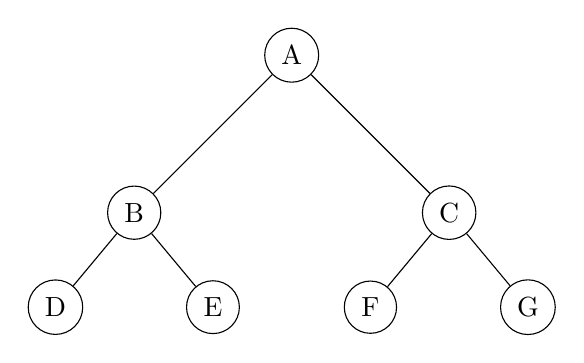
\begin{tikzpicture}[
level 1/.style={level distance=20mm, sibling distance=40mm},
level 2/.style={level distance=12mm, sibling distance=20mm},
every node/.style={circle,draw}
]
\node {A}
child {
    node {B}
    child {node {D}}
    child {node {E}}
}
child {
    node {C}
    child {node {F}}
    child {node {G}}
};
\end{tikzpicture}

The topmost node is called the \textbf{root}. A node with no children is called a \textbf{leaf}. 
Every node together with all of its descendants forms a \textbf{subtree}.

\subsection{Tree Traversal}
A traversal specifies the order in which nodes are visited. The most important traversal for 
our purposes is the \textbf{In-Order Traversal}.

\begin{center}
\begin{minipage}{0.9\linewidth}
\begin{framed}
\begin{Verbatim}
IOT(x)
{
    if (x is null)
        return

    IOT(x.left)
    print(x.value)
    IOT(x.right)
}

IOT(root) \\starting the recursive traversal from the root
\end{Verbatim}
\vspace{-4mm}
\end{framed}
\end{minipage}
\end{center}

\vspace{1em}
\begin{center}
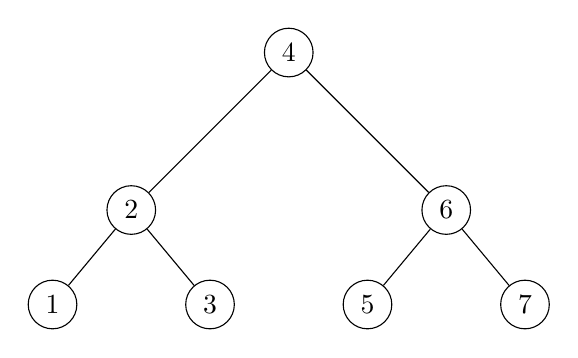
\begin{tikzpicture}[
level 1/.style={level distance=20mm, sibling distance=40mm},
level 2/.style={level distance=12mm, sibling distance=20mm},
every node/.style={circle,draw}
]
\node {4}
child {
    node {2}
    child {node {1}}
    child {node {3}}
}
child {
    node {6}
    child {node {5}}
    child {node {7}}
};
\end{tikzpicture}
\end{center}

Convince yourself that the output for the above tree will be \texttt{1 2 3 4 5 6 7}. In-Order Traversal 
is most commonly seen in \texttt{Depth-First Search}, popularly known as \texttt{DFS}. 

\subsection{Binary Search Trees}

The value stored at each node is referred to as its \textbf{key}. A binary search tree (BST) is a 
binary tree in which every non-leaf node satisfies the following properties:
\begin{itemize}
\item All keys in the left subtree are smaller than the node's key.
\item All keys in the right subtree are larger than the node's key.
\end{itemize}

Any tree which has the above two properties is said to have the \textbf{BST} property.
\begin{center}
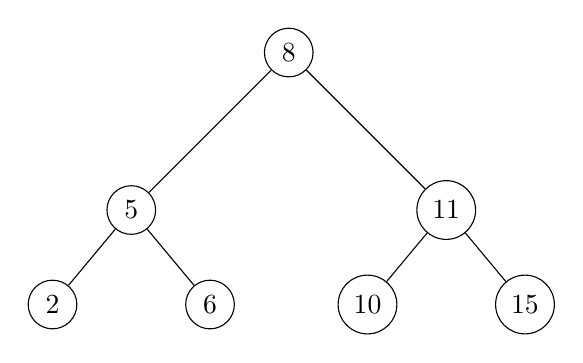
\begin{tikzpicture}[
level 1/.style={level distance=20mm, sibling distance=40mm},
level 2/.style={level distance=12mm, sibling distance=20mm},
every node/.style={circle,draw}
]
\node {8}
child {
    node {5}
    child {node {2}}
    child {node {6}}
}
child {
    node {11}
    child {node {10}}
    child {node {15}}
};
\end{tikzpicture}
\end{center}

With some thought it can be proved that an In-Order Traversal of a BST lists all keys in sorted order.

\subsubsection*{Search}
Searching for a key proceeds exactly as in binary search. At each node we 
compare the desired key with the current key and move either left or right. 
If the tree is balanced, the tree is the same as the recursion tree of a normal binary search 
on a sorted array $\dots$ \\

\begin{center}
\begin{minipage}{0.9\linewidth}
\begin{framed}
\begin{Verbatim}
Search(key,node)
{
    if (node is null)
        return false

    if(key < node.value)
        return Search(key,node.left)
    if(node.value == key)
        return true
    if(key > node.value)
        return Search(key,node.right)
}

Search(x,root) \\Search the key x, starting from the root
\end{Verbatim}
\vspace{-4mm}
\end{framed}
\end{minipage}
\end{center}

Let us say we are searching for $6$ in the tree we saw earlier. 
\begin{center}
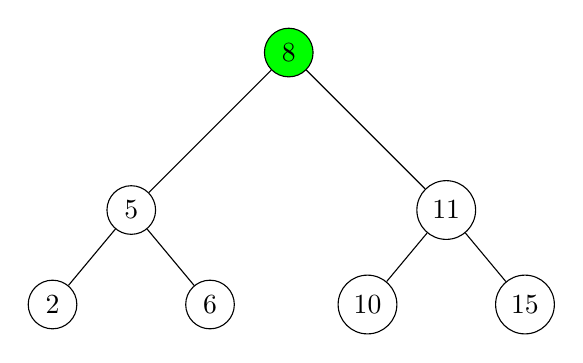
\begin{tikzpicture}[
level 1/.style={level distance=20mm, sibling distance=40mm},
level 2/.style={level distance=12mm, sibling distance=20mm},
every node/.style={circle,draw}
]
\node (1)[fill=green]{8}
child{
    node (2){5}
    child {
        node (4){2}
    }
    child {
        node (5){6}
    }
}
child {
    node (3){11}
    child {node (6){10}}
    child {node (7){15}}
};

\end{tikzpicture}
\end{center}


Since $8$ is greater than $6$, we move left.\\
\begin{center}
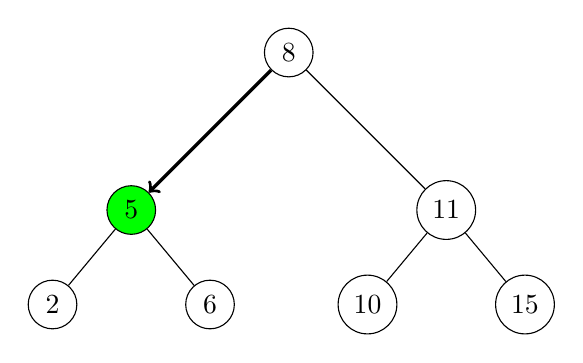
\begin{tikzpicture}[
level 1/.style={level distance=20mm, sibling distance=40mm},
level 2/.style={level distance=12mm, sibling distance=20mm},
every node/.style={circle,draw}
]
\node (1){8}
child{
    node (2)[fill=green]{5}
    child {
        node (4){2}
    }
    child {
        node (5){6}
    }
}
child {
    node (3){11}
    child {node (6){10}}
    child {node (7){15}}
};

\draw[white,very thick,->] (1) -- (2);
\draw[black,very thick,->] (1) -- (2);
\end{tikzpicture}
\end{center}


Since $5$ is less than $6$, we move right.\\
\begin{center}
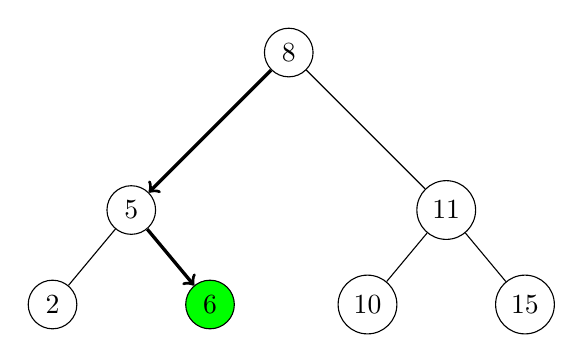
\begin{tikzpicture}[
level 1/.style={level distance=20mm, sibling distance=40mm},
level 2/.style={level distance=12mm, sibling distance=20mm},
every node/.style={circle,draw}
]
\node (1){8}
child{
    node (2){5}
    child {
        node (4){2}
    }
    child {
        node (5)[fill=green]{6}
    }
}
child {
    node (3){11}
    child {node (6){10}}
    child {node (7){15}}
};

\draw[white,very thick,->] (1) -- (2);
\draw[black,very thick,->] (1) -- (2);
\draw[white,very thick,->] (2) -- (5);
\draw[black,very thick,->] (2) -- (5);
\end{tikzpicture}
\end{center}

We found it! If we had instead been looking for $7$, we would have taken the same path and ended 
up at the right child of leaf $6$ (which is of course, an empty node) so we would have concluded that $7$ is not 
in the tree. 

\subsubsection*{Insertion}
Insertion is similar to binary search. At each node we compare the key to be inserted with the 
current key and move either left or right. If we find the key in the tree, we do nothing. If we reach an empty 
node we insert the key there.

\begin{center}
\begin{minipage}{0.9\linewidth}
\begin{framed}
\begin{Verbatim}
Insert(key,node)
{
    if (node is null)
    {
        node = new Node(value=key, left=null, right=null)
        return
    }

    if(key < node.value)
        Insert(key,node.left)

    if(node.value == key)
        return

    if(key > node.value)
        Insert(key,node.right)
}

Insert(x,root) \\Insert the key x, recurse starting from the root
\end{Verbatim}
\vspace{-4mm}
\end{framed}
\end{minipage}
\end{center}


Let us say we want to insert $7$ in the tree we saw earlier. \\

\begin{center}
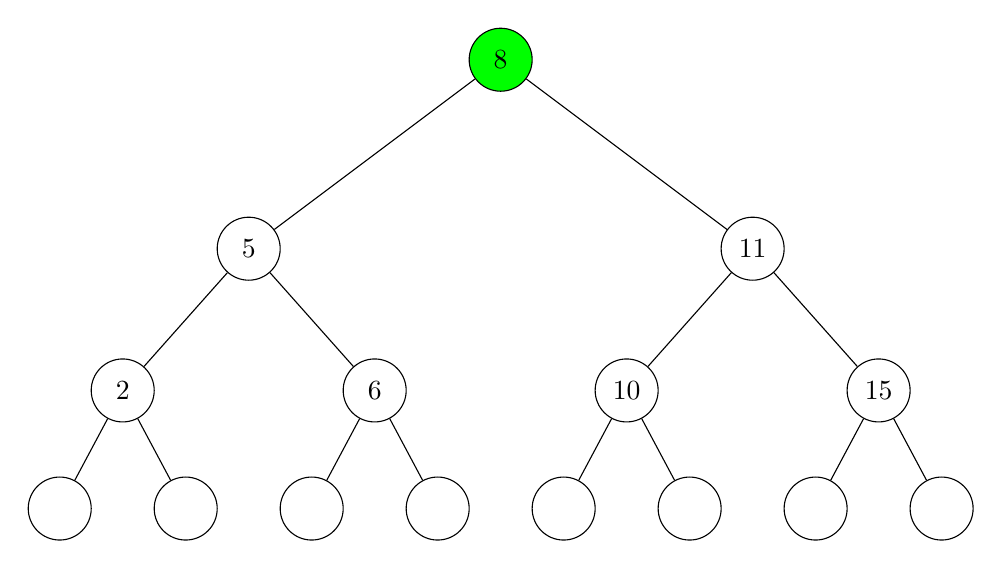
\begin{tikzpicture}[
level 1/.style={level distance=24mm,sibling distance=64mm},
level 2/.style={level distance=18mm,sibling distance=32mm},
level 3/.style={level distance=15mm,sibling distance=16mm},
every node/.style={circle,draw,minimum size=8mm}
]
\node (1)[fill=green]{8}
child{
    node (2){5}
    child {
        node (4){2}
        child { node (8){} }
        child { node (9){} }
    }
    child {
        node (5){6}
        child { node (10){} }
        child { node (11){} }
    }
}
child {
    node (3){11}
    child {
        node (6){10}
        child { node (12){} }
        child { node (13){} }
    }
    child {
        node (7){15}
        child { node (14){} }
        child { node (15){} }
    }
};
\end{tikzpicture}
\end{center}


Since $8$ is greater than $7$, we move left.\\

\begin{center}
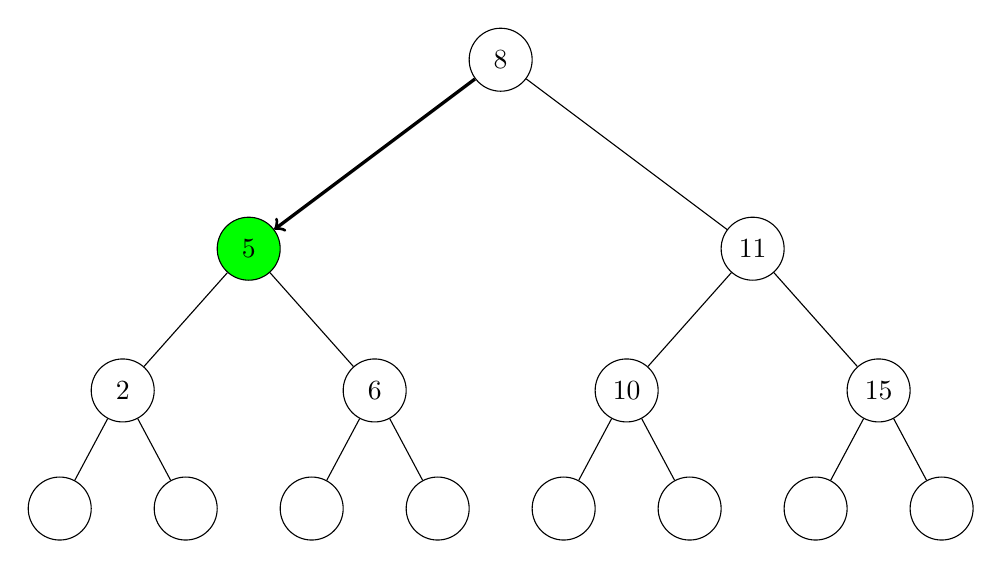
\begin{tikzpicture}[
level 1/.style={level distance=24mm,sibling distance=64mm},
level 2/.style={level distance=18mm,sibling distance=32mm},
level 3/.style={level distance=15mm,sibling distance=16mm},
every node/.style={circle,draw,minimum size=8mm}
]
\node (1){8}
child{
    node [fill=green](2){5}
    child {
        node (4){2}
        child { node (8){} }
        child { node (9){} }
    }
    child {
        node (5){6}
        child { node (10){} }
        child { node (11){} }
    }
}
child {
    node (3){11}
    child {
        node (6){10}
        child { node (12){} }
        child { node (13){} }
    }
    child {
        node (7){15}
        child { node (14){} }
        child { node (15){} }
    }
};
\draw[white,very thick,->] (1) -- (2); 
\draw[black,very thick,->] (1) -- (2); 
\end{tikzpicture}
\end{center}

Since $5$ is less than $7$, we move right.\\

\begin{center}
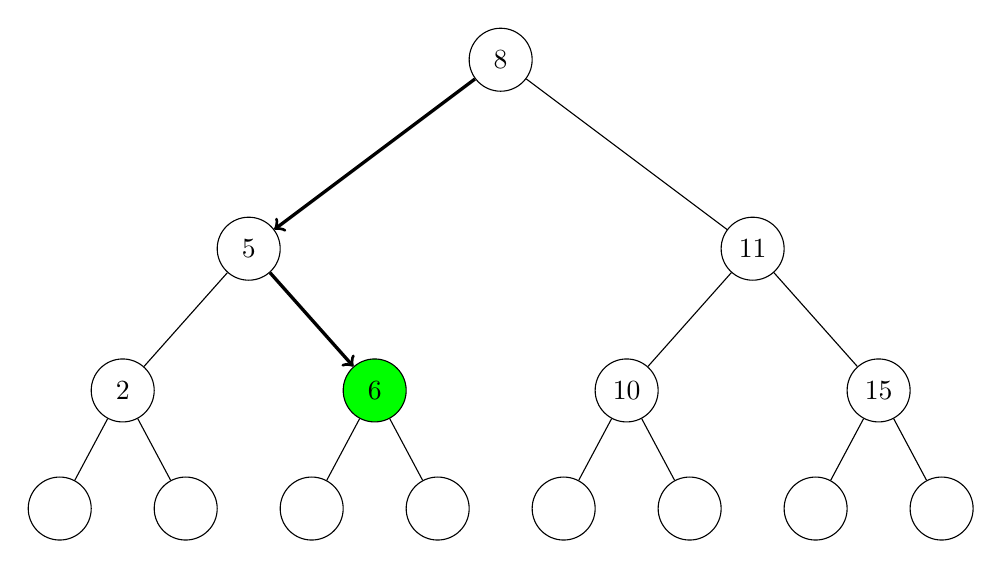
\begin{tikzpicture}[
level 1/.style={level distance=24mm,sibling distance=64mm},
level 2/.style={level distance=18mm,sibling distance=32mm},
level 3/.style={level distance=15mm,sibling distance=16mm},
every node/.style={circle,draw,minimum size=8mm}
]
\node (1){8}
child{
    node (2){5}
    child {
        node (4){2}
        child { node (8){} }
        child { node (9){} }
    }
    child {
        node [fill=green](5){6}
        child { node (10){} }
        child { node (11){} }
    }
}
child {
    node (3){11}
    child {
        node (6){10}
        child { node (12){} }
        child { node (13){} }
    }
    child {
        node (7){15}
        child { node (14){} }
        child { node (15){} }
    }
};
\draw[white,very thick,->] (1) -- (2); 
\draw[black,very thick,->] (1) -- (2); 
\draw[white,very thick,->] (2) -- (5); 
\draw[black,very thick,->] (2) -- (5); 
\end{tikzpicture}
\end{center}

Since $6$ is less than $7$, we move right.\\

\begin{center}
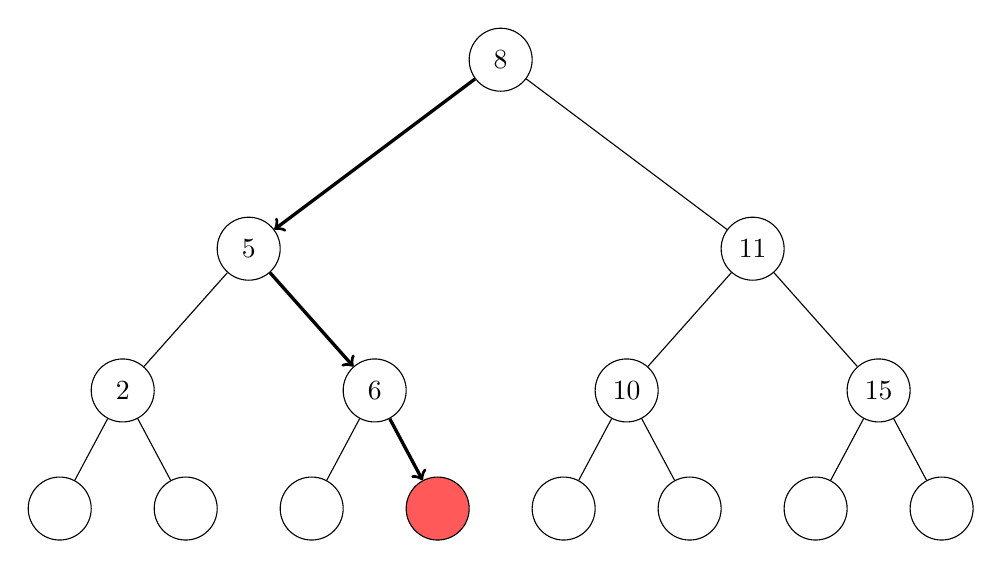
\begin{tikzpicture}[
level 1/.style={level distance=24mm,sibling distance=64mm},
level 2/.style={level distance=18mm,sibling distance=32mm},
level 3/.style={level distance=15mm,sibling distance=16mm},
every node/.style={circle,draw,minimum size=8mm}
]
\node (1){8}
child{
    node (2){5}
    child {
        node (4){2}
        child { node (8){} }
        child { node (9){} }
    }
    child {
        node (5){6}
        child { node (10){} }
        child { node (11)[fill=red!65]{} }
    }
}
child {
    node (3){11}
    child {
        node (6){10}
        child { node (12){} }
        child { node (13){} }
    }
    child {
        node (7){15}
        child { node (14){} }
        child { node (15){} }
    }
};
\draw[white,very thick,->] (1) -- (2); 
\draw[black,very thick,->] (1) -- (2); 
\draw[white,very thick,->] (2) -- (5); 
\draw[black,very thick,->] (2) -- (5); 
\draw[white,very thick,->] (5) -- (11);
\draw[black,very thick,->] (5) -- (11);
\end{tikzpicture}
\end{center}

Since the node is empty, we create a new node and put $7$ in it.\\

\begin{center}
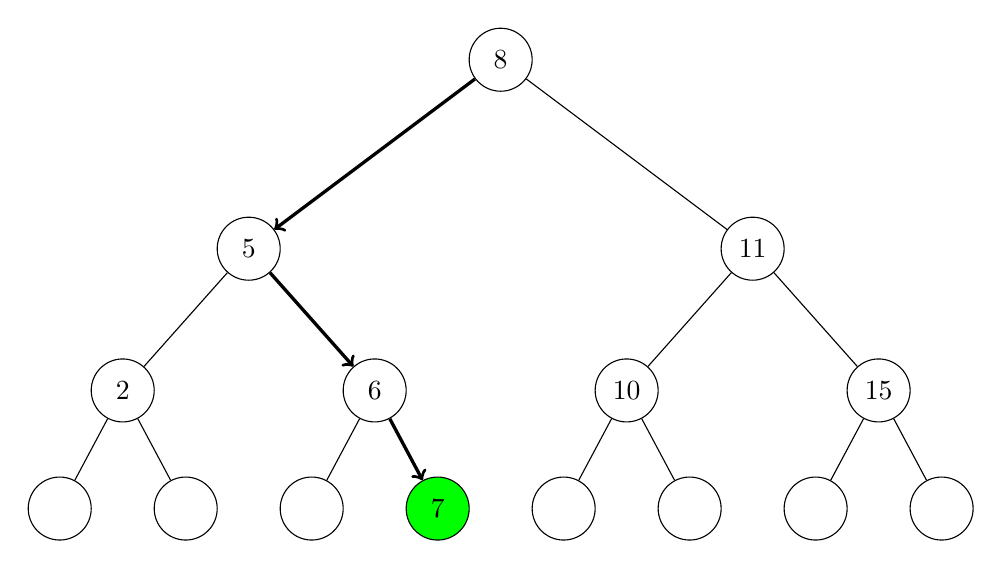
\begin{tikzpicture}[
level 1/.style={level distance=24mm,sibling distance=64mm},
level 2/.style={level distance=18mm,sibling distance=32mm},
level 3/.style={level distance=15mm,sibling distance=16mm},
every node/.style={circle,draw,minimum size=8mm}
]
\node (1){8}
child{
    node (2){5}
    child {
        node (4){2}
        child { node (8){} }
        child { node (9){} }
    }
    child {
        node (5){6}
        child { node (10){} }
        child { node (11)[fill=green]{7} }
    }
}
child {
    node (3){11}
    child {
        node (6){10}
        child { node (12){} }
        child { node (13){} }
    }
    child {
        node (7){15}
        child { node (14){} }
        child { node (15){} }
    }
};
\draw[white,very thick,->] (1) -- (2); 
\draw[black,very thick,->] (1) -- (2); 
\draw[white,very thick,->] (2) -- (5); 
\draw[black,very thick,->] (2) -- (5); 
\draw[white,very thick,->] (5) -- (11);
\draw[black,very thick,->] (5) -- (11);
\end{tikzpicture}
\end{center}


\subsection{Balancing}

The efficiency of a BST depends on its height. If the tree has height \(h\), 
then search, insertion and deletion requires worst-case \(\Theta(h)\) time. 
Ideally we would like $h=\Theta(\log n)$ where \(n\) is the number of stored keys. Unfortunately, a 
BST can become highly unbalanced. For example, inserting the keys $1, 2, 3, 4, \dots n$ in this order 
produces a tree with height \(n\). 


\begin{center}
\begin{tikzpicture}[
level distance=12mm,
every node/.style={circle,draw,minimum size=8mm}
]
\node {1}
child[missing]
child {
    node {2}
    child[missing]
    child {
        node {3}
        child[missing]
        child {
            node {4}
            child[missing]
            child {node {5}}
        }
    }
};
\end{tikzpicture}
\end{center}

\begin{center}
\vspace{-0.3em}
\textbf{Example with $\mathbf{n=5}$}
\end{center}
\vspace{1em}

This tree is essentially a linked list. Its height is \(n\) and consequently all operations 
require \(\Theta(n)\) time. To avoid this degeneration we need a 
mechanism for changing the shape of a tree while preserving the BST property.


\subsection{Min-Heaps}

A min-heap is a binary tree that satisfies two important properties:

\begin{enumerate}
\item \textbf{Complete}: Every level is completely filled except possibly the last 
level, which is filled from left to right. 

\begin{center}
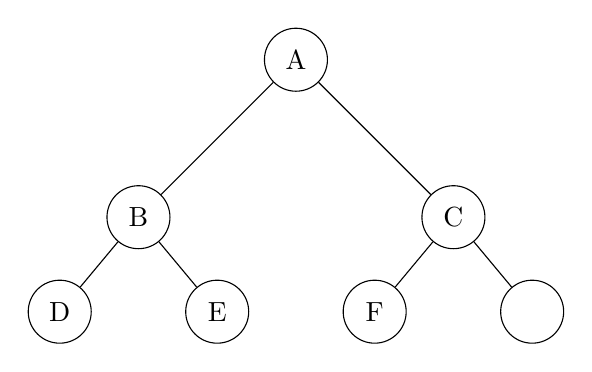
\begin{tikzpicture}[
minimum size=8mm,
level 1/.style={level distance=20mm, sibling distance=40mm},
level 2/.style={level distance=12mm, sibling distance=20mm},
every node/.style={circle,draw}
]
\node {A}
child {
node {B}
child {node {D}}
child {node {E}}
}
child {
node {C}
child {node {F}}
child {node {}}
};
\end{tikzpicture}
\end{center}

The above figure shows a complete binary tree.

\item \textbf{Min-Heap Property}:
\begin{itemize}
\item In a \textbf{Min-Heap}, every node is less than or equal to its children.

\begin{center}
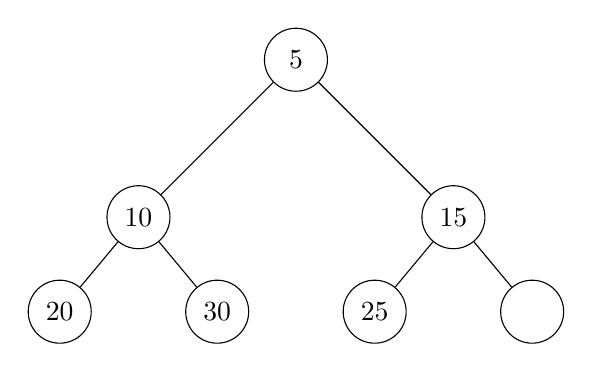
\begin{tikzpicture}[
minimum size=8mm,
level 1/.style={level distance=20mm, sibling distance=40mm},
level 2/.style={level distance=12mm, sibling distance=20mm},
every node/.style={circle,draw}
]
\node {5}
child{
	node{10}
	child {
		node {20}
	}
	child {
		node {30}
	}
}
child {
	node {15}
	child {
		node {25}
	}
	child {
		node {}
	}
};
\end{tikzpicture}
\end{center}

The above figure shows a min-heap. It can be easily proved that the root has the smallest value in a 
min-heap. 

\end{itemize}
\end{enumerate}

A min-heap can support the \texttt{push} and \texttt{pop} operations.

\subsubsection*{Popping}
The \texttt{pop()} function returns the root of the heap and removes it from the heap. To maintain the heap, 
we must then move some values up the tree. Logically, the smaller child should be moved up to the root. 
This creates a vacancy in the subtree in which the child was pushed up. That subtree now behaves like a 
smaller version of the original problem -- a heap from which the root was removed. So we can recursively 
push the smaller child up until we hit empty node.

\begin{center}
\begin{minipage}{0.9\linewidth}
\begin{framed}
\begin{Verbatim}
pop(root)
{
	ans=root.value
	root.value=null
	if(root.left < root.right)
		root.value=pop(root.leftChild)
	else
		pop(root.rightChild)
	return ans
}
\end{Verbatim}
\vspace{-4mm}
\end{framed}
\end{minipage}
\end{center}

\subsubsection*{Pushing}

The \texttt{push()} function adds a new value to the heap by putting the new value at the 
bottom of the tree and then pushing it up until heap property is restored. 

\begin{center}
\begin{minipage}{0.9\linewidth}
\begin{framed}
\begin{Verbatim}
push(x)
{
	curr=bottomLeftMostNode
	curr.value=x

	while(curr.value<curr.parent.value)
	{
		swap(curr.value,curr.parent.value)
		curr=curr.parent
	}
}
\end{Verbatim}
\vspace{-4mm}
\end{framed}
\end{minipage}
\end{center}

Let us insert $7$ into the following min-heap.

\begin{center}
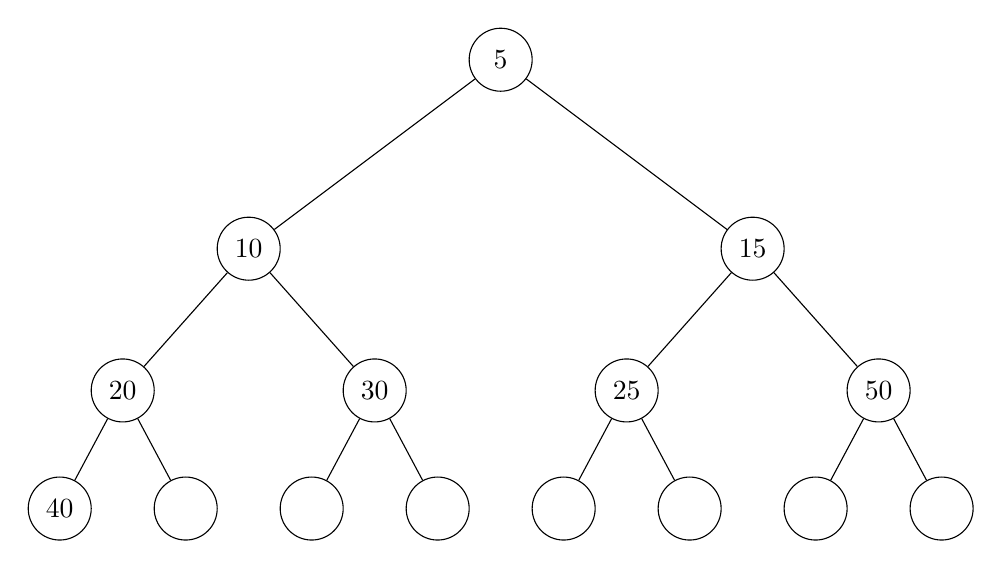
\begin{tikzpicture}[
minimum size=8mm,
level 1/.style={level distance=24mm,sibling distance=64mm},
level 2/.style={level distance=18mm,sibling distance=32mm},
level 3/.style={level distance=15mm,sibling distance=16mm},
every node/.style={circle,draw}
]
\node{5}
child{
	node{10}
	child{ 
		node{20}
		child{node{40}}
		child{node{}}
	}
	child {
		node{30}
		child{node{}}
		child{node{}}
	}
}
child {
	node {15}
	child {
		node{25}
		child{node{}}
		child{node{}}
	}
	child {
		node{50}
		child{node{}}
		child{node{}}
	}
};
\end{tikzpicture}
\end{center}


Insert 7 in bottom left most node. We detect the violation $20>7$.
\begin{center}
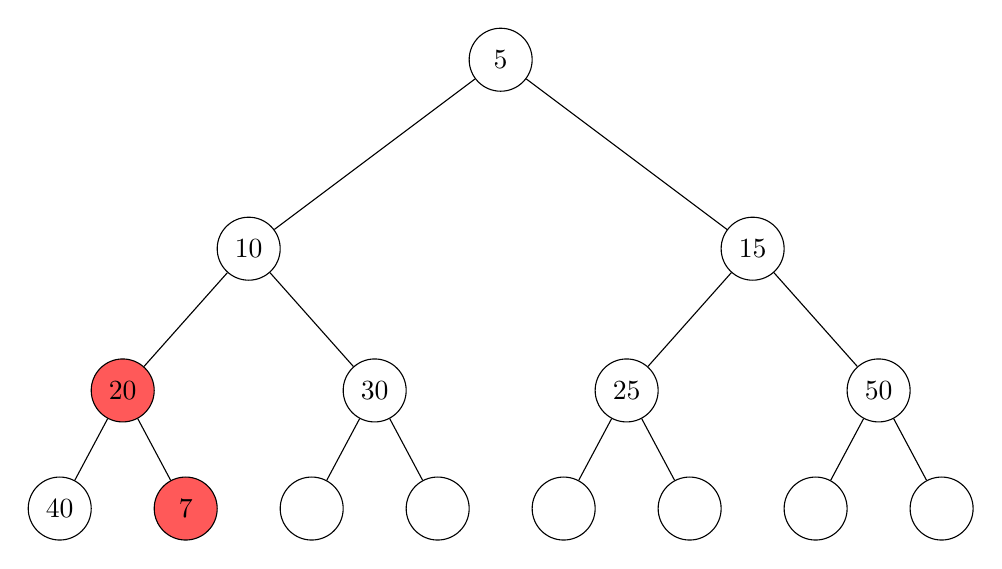
\begin{tikzpicture}[
minimum size=8mm,
level 1/.style={level distance=24mm,sibling distance=64mm},
level 2/.style={level distance=18mm,sibling distance=32mm},
level 3/.style={level distance=15mm,sibling distance=16mm},
every node/.style={circle,draw}
]
\node{5}
child{
	node{10}
	child{ 
		node[fill=red!65](1){20}
		child{node{40}}
		child{node[fill=red!65](2){7}}
	}
	child {
		node{30}
		child{node{}}
		child{node{}}
	}
}
child {
	node {15}
	child {
		node{25}
		child{node{}}
		child{node{}}
	}
	child {
		node{50}
		child{node{}}
		child{node{}}
	}
};
\end{tikzpicture}
\end{center}


We swap them to solve the violation.
\begin{center}
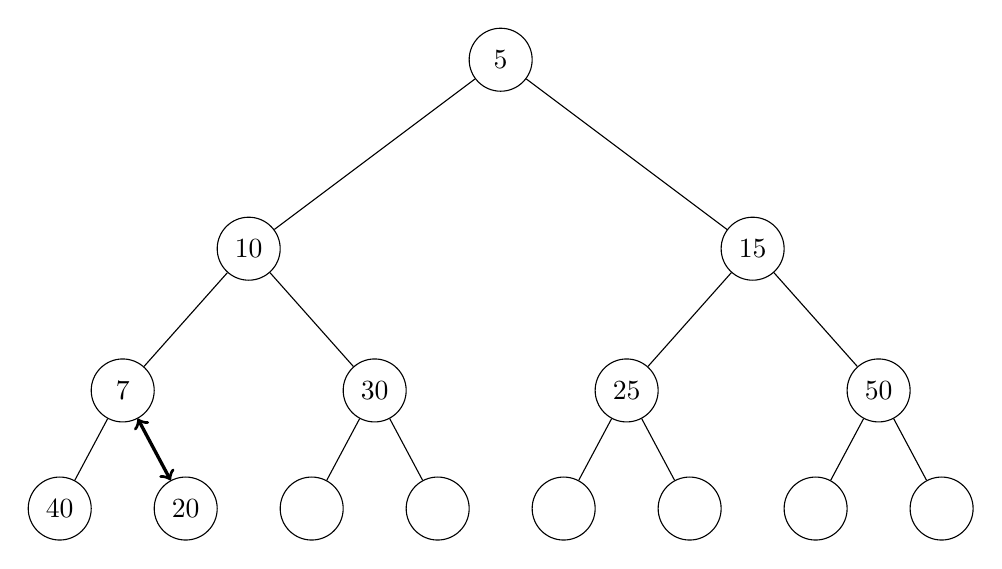
\begin{tikzpicture}[
minimum size=8mm,
level 1/.style={level distance=24mm,sibling distance=64mm},
level 2/.style={level distance=18mm,sibling distance=32mm},
level 3/.style={level distance=15mm,sibling distance=16mm},
every node/.style={circle,draw}
]
\node{5}
child{
	node{10}
	child{ 
		node(1){7}
		child{node{40}}
		child{node(2){20}}
	}
	child {
		node{30}
		child{node{}}
		child{node{}}
	}
}
child {
	node {15}
	child {
		node{25}
		child{node{}}
		child{node{}}
	}
	child {
		node{50}
		child{node{}}
		child{node{}}
	}
};
\draw[<->,very thick] (1)--(2);
\end{tikzpicture}
\end{center}



We detect the violation $10>7$.
\begin{center}
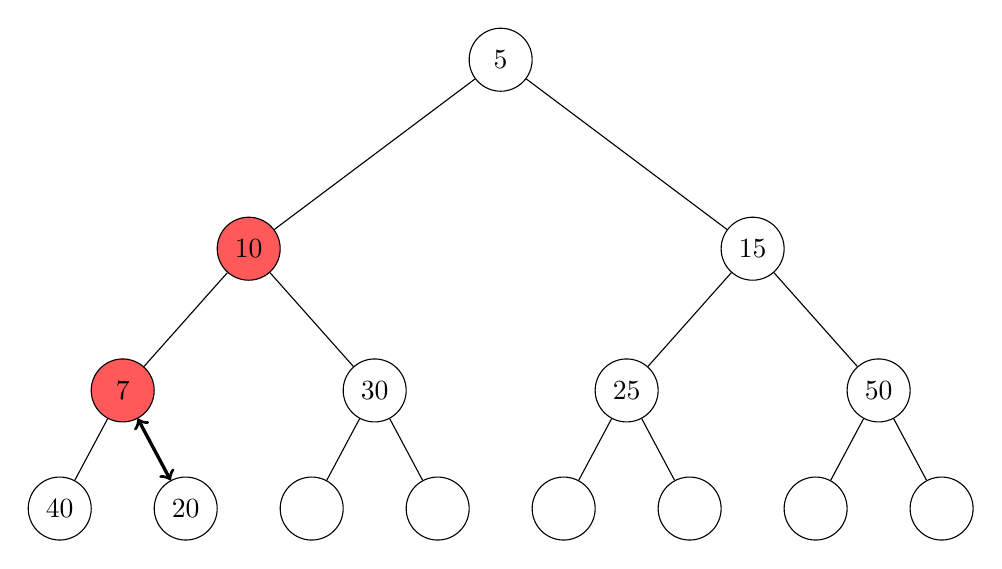
\begin{tikzpicture}[
minimum size=8mm,
level 1/.style={level distance=24mm,sibling distance=64mm},
level 2/.style={level distance=18mm,sibling distance=32mm},
level 3/.style={level distance=15mm,sibling distance=16mm},
every node/.style={circle,draw}
]
\node{5}
child{
	node[fill=red!65]{10}
	child{ 
		node(1)[fill=red!65]{7}
		child{node{40}}
		child{node(2){20}}
	}
	child {
		node{30}
		child{node{}}
		child{node{}}
	}
}
child {
	node {15}
	child {
		node{25}
		child{node{}}
		child{node{}}
	}
	child {
		node{50}
		child{node{}}
		child{node{}}
	}
};
\draw[<->,very thick] (1)--(2);
\end{tikzpicture}
\end{center}


We swap them to solve the violation.
\begin{center}
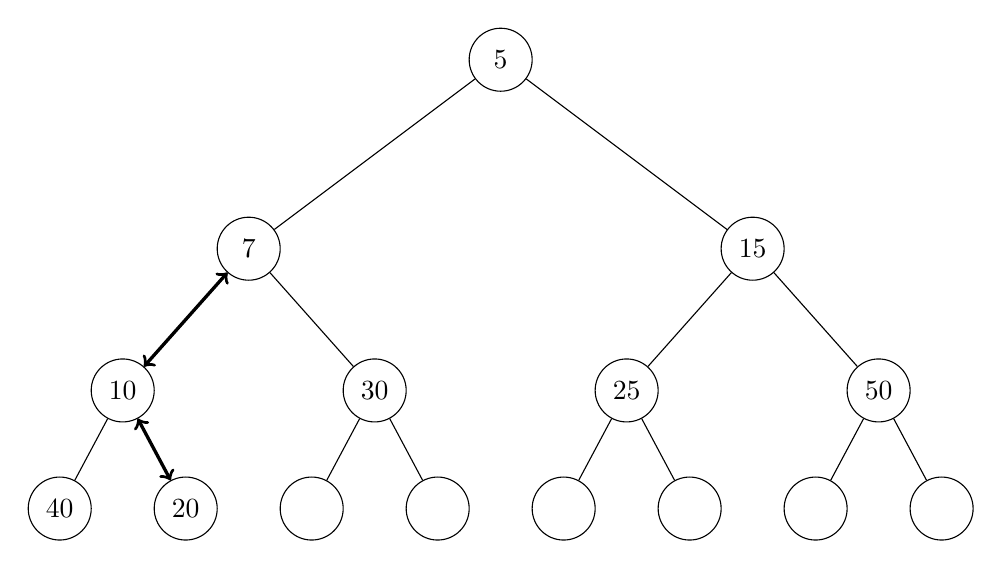
\begin{tikzpicture}[
minimum size=8mm,
level 1/.style={level distance=24mm,sibling distance=64mm},
level 2/.style={level distance=18mm,sibling distance=32mm},
level 3/.style={level distance=15mm,sibling distance=16mm},
every node/.style={circle,draw}
]
\node{5}
child{
	node(3){7}
	child{ 
		node(1){10}
		child{node{40}}
		child{node(2){20}}
	}
	child {
		node{30}
		child{node{}}
		child{node{}}
	}
}
child {
	node {15}
	child {
		node{25}
		child{node{}}
		child{node{}}
	}
	child {
		node{50}
		child{node{}}
		child{node{}}
	}
};
\draw[<->,very thick] (1)--(2);
\draw[<->,very thick] (3)--(1);
\end{tikzpicture}
\end{center}


It can be proved that when there is no more violation involving the inserted value, there is no more 
violation in the tree. Thus the heap property is restored. 


\subsection{Rotations}
These are operations that transform a tree into another tree with the same inorder traversal. From an 
undirected graph perspective the only change that occurs is one edge is deleted and one is added. But from 
a rooted tree perspective 2 father-child relationships are changed. There are two types of rotations (left 
and right) which are inverse of each other.

\subsubsection*{Left Rotation}
\vspace{1em}
\begin{center}
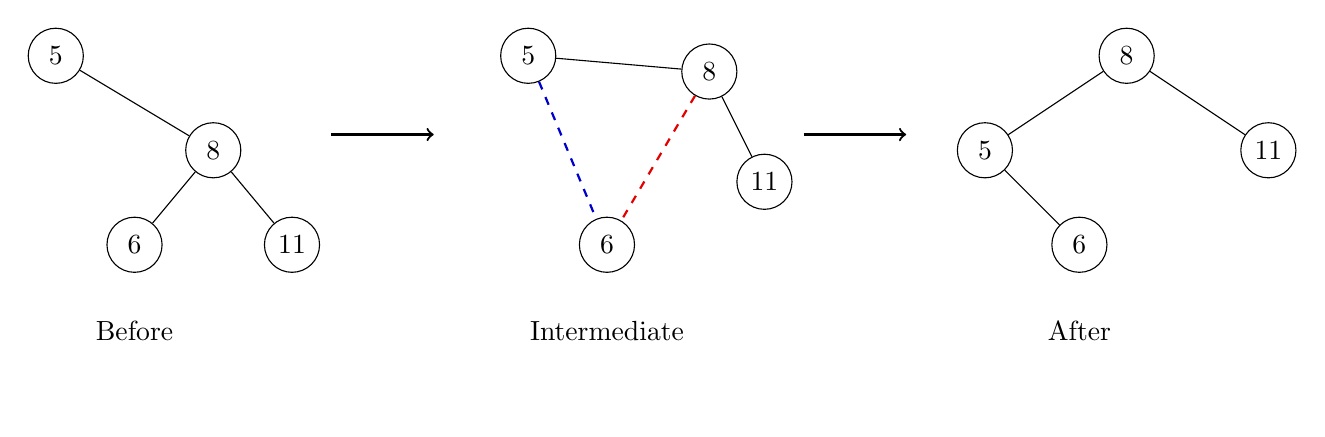
\begin{tikzpicture}[
every node/.style={
    circle,
    draw,
    minimum size=7mm,
    inner sep=0pt
},
level distance=12mm,
sibling distance=18mm
]

%---------------- Original ----------------
\begin{scope}
\node (x) at (0,0) {5};
\node (y) at (2,-1.2) {8};
\node (a) at (1,-2.4) {6};
\node (b) at (3,-2.4) {11};

\draw (x)--(y);
\draw (y)--(a);
\draw (y)--(b);

\node[draw=none] at (1,-3.5) {Before};
\end{scope}

%---------------- Intermediate ----------------
\begin{scope}[xshift=6cm]
\node (x) at (0,0) {5};
\node (y) at (2.3,-0.2) {8};
\node (a) at (1,-2.4) {6};
\node (b) at (3,-1.6) {11};

\draw[dashed,thick,blue!80!black] (x)--(a);
\draw (x)--(y);
\draw[dashed,thick,red!90!black] (y)--(a);
\draw (y)--(b);

\node[draw=none] at (1,-3.5) {Intermediate};
\end{scope}

%---------------- Final ----------------
\begin{scope}[xshift=13cm]
\node (y) at (0.6,0) {8};
\node (x) at (-1.2,-1.2) {5};
\node (a) at (0,-2.4) {6};
\node (b) at (2.4,-1.2) {11};

\draw (y)--(x);
\draw (y)--(b);
\draw (x)--(a);

\node[draw=none] at (0,-3.5) {After};
\end{scope}

\draw[->,thick] (3.5,-1) -- (4.8,-1);
\draw[->,thick] (9.5,-1) -- (10.8,-1);

\end{tikzpicture}
\end{center}

\subsubsection*{Right Rotation}
\vspace{1em}
\begin{center}
\begin{tikzpicture}[
every node/.style={
    circle,
    draw,
    minimum size=7mm,
    inner sep=0pt
},
level distance=12mm,
sibling distance=18mm
]

%---------------- Original ----------------
\begin{scope}
\node (y) at (0.6,0) {8};
\node (x) at (-1.2,-1.2) {5};
\node (a) at (0,-2.4) {6};
\node (b) at (2.4,-1.2) {11};

\draw (y)--(x);
\draw (y)--(b);
\draw (x)--(a);

\node[draw=none] at (0,-3.5) {Before};
\end{scope}

\draw[->,thick] (3.5,-1) -- (4.8,-1);
\draw[->,thick] (9.5,-1) -- (10.8,-1);

%---------------- Intermediate ----------------
\begin{scope}[xshift=6cm]
\node (x) at (0,0) {5};
\node (y) at (2.3,-0.2) {8};
\node (a) at (1,-2.4) {6};
\node (b) at (3,-1.6) {11};

\draw[dashed,thick,red!90!black] (x)--(a);
\draw (x)--(y);
\draw[dashed,thick,blue!80!black] (y)--(a);
\draw (y)--(b);

\node[draw=none] at (1,-3.5) {Intermediate};
\end{scope}

%---------------- Final ----------------
\begin{scope}[xshift=13cm]
\node (x) at (0,0) {5};
\node (y) at (2,-1.2) {8};
\node (a) at (1,-2.4) {6};
\node (b) at (3,-2.4) {11};

\draw (x)--(y);
\draw (y)--(a);
\draw (y)--(b);

\node[draw=none] at (1,-3.5) {After};
\end{scope}

\end{tikzpicture}
\end{center}

Rotations can also fix heap violations the same way swaps did with the added benefit of preserving 
in-order traversal. A violation with right child and parent can be fixed with a left rotation at the parent 
and vice-versa. 

\begin{center}
\begin{tikzpicture}[
every node/.style={
    circle,
    draw,
    minimum size=7mm,
    inner sep=0pt
},
level distance=12mm,
sibling distance=18mm
]

%---------------- Original ----------------
\begin{scope}
\node (x) at (0,0) [fill=RED]{8};
\node (y) at (2,-1.2) [fill=RED]{5};
\node (a) at (1,-2.4) {6};
\node (b) at (3,-2.4) {11};

\draw (x)--(y);
\draw (y)--(a);
\draw (y)--(b);

\node[draw=none] at (1,-3.5) {Before};
\end{scope}

%---------------- Final ----------------
\begin{scope}[xshift=9cm]
\node (y) at (0.6,0) {5};
\node (x) at (-1.2,-1.2) {8};
\node (a) at (0,-2.4) {6};
\node (b) at (2.4,-1.2) {11};

\draw (y)--(x);
\draw (y)--(b);
\draw (x)--(a);

\node[draw=none] at (0,-3.5) {After};
\end{scope}

\node [draw=none] (c) at (5.3,-0.8) {Left Rotation};
\draw[->,thick] (3.8,-1.2) -- (6.8,-1.2);

\end{tikzpicture}
\end{center}

\begin{center}
\begin{tikzpicture}[
every node/.style={
    circle,
    draw,
    minimum size=7mm,
    inner sep=0pt
},
level distance=12mm,
sibling distance=18mm
]

%---------------- Original ----------------
\begin{scope}
\node (y) at (0.6,0) {5};
\node (x) at (-1.2,-1.2) [fill=RED]{8};
\node (a) at (0,-2.4) [fill=RED]{6};
\node (b) at (2.4,-1.2) {11};

\draw (y)--(x);
\draw (y)--(b);
\draw (x)--(a);

\node[draw=none] at (0,-3.5) {Before};
\end{scope}


%---------------- Final ----------------

\begin{scope}[xshift=8.5cm]
\node (y) at (0.6,0) {5};
\node (x) at (-2.0,-2.4) {8};
\node (a) at (-1.2,-1.2) {6};
\node (b) at (2.4,-1.2) {11};

\draw (y)--(a);
\draw (y)--(b);
\draw (x)--(a);

\node[draw=none] at (0,-3.5) {After};
\end{scope}

\node [draw=none] (c) at (4.7,-0.8) {Left Rotation};
\draw[->,thick] (3.2,-1.2) -- (6.2,-1.2);

\end{tikzpicture}
\end{center}

Similar to Bubble Sort and the concept of inversions, we can look at the original tree as having $2$ 
violations -- $8$ was above both $5$ and $6$ in the tree. Each rotation fixes exactly one of these 
violations just like each swap in Bubble Sort.

\subsection{Treaps}

Each node stores a key and along with it a random priority. 

\[
\texttt{Node.value=(key,priority)}
\]


A treap simultaneously satisfies:
\begin{enumerate}
\item The \textbf{BST property} with respect to keys.
\item The \textbf{min-heap property} with respect to priorities.
\end{enumerate}


\begin{center}
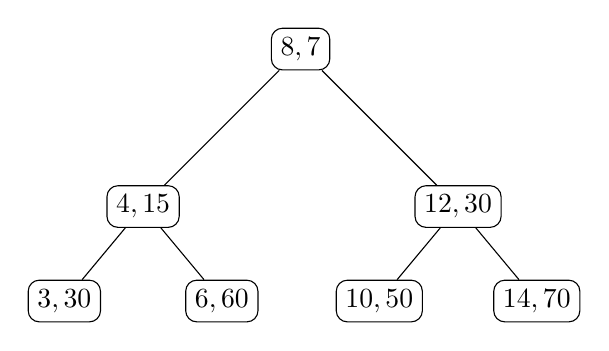
\begin{tikzpicture}[
minimum size=5mm,
level 1/.style={level distance=20mm, sibling distance=40mm},
level 2/.style={level distance=12mm, sibling distance=20mm},
every node/.style={draw,rounded corners}
]
\node {$8,7$}
child {
    node {$4,15$}
    child {node {$3,30$}}
    child {node {$6,60$}}
}
child {
    node {$12,30$}
    child {node {$10,50$}}
    child {node {$14,70$}}
};
\end{tikzpicture}
\end{center}

The above figure shows a treap in which the first value is the key and the second is the priority.

\subsubsection*{Insertion}

Insertion in a treap proceeds in two phases. First, we insert the new key exactly as in a 
binary search tree. Then, if the heap property is violated, we restore it using rotations. Consider the 
following treap, where each node stores a pair $(\text{key},\text{priority})$ and priorities 
satisfy the min-heap property.

\begin{center}
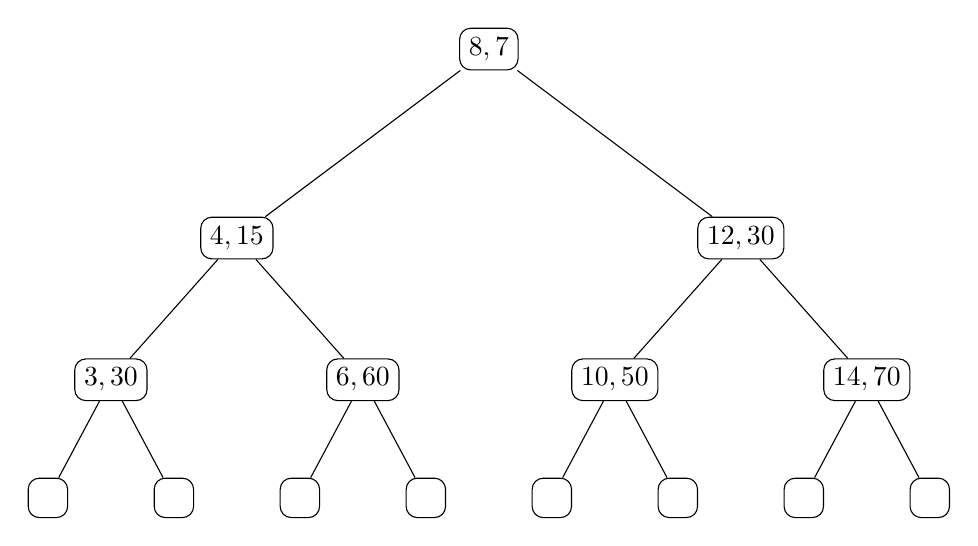
\begin{tikzpicture}[
minimum size=5mm,
level 1/.style={level distance=24mm,sibling distance=64mm},
level 2/.style={level distance=18mm,sibling distance=32mm},
level 3/.style={level distance=15mm,sibling distance=16mm},
every node/.style={draw,rounded corners}
]
\node {$8,7$}
child {
    node {$4,15$}
    child {
		node {$3,30$}
		child{node{}}
		child{node{}}
	}
    child {
		node {$6,60$}
		child{node{}}
		child{node{}}
	}
}
child {
    node {$12,30$}
    child {
		node {$10,50$}
		child{node{}}
		child{node{}}
	}
    child {
		node {$14,70$}
		child{node{}}
		child{node{}}
	}
};
\end{tikzpicture}
\end{center}

Suppose we wish to insert the node $(5,10)$.

\paragraph{Step 1: BST Insertion}

Ignoring priorities, we first insert the key according to the BST property -- the new node 
becomes the left child of $(6,60)$.

\begin{center}
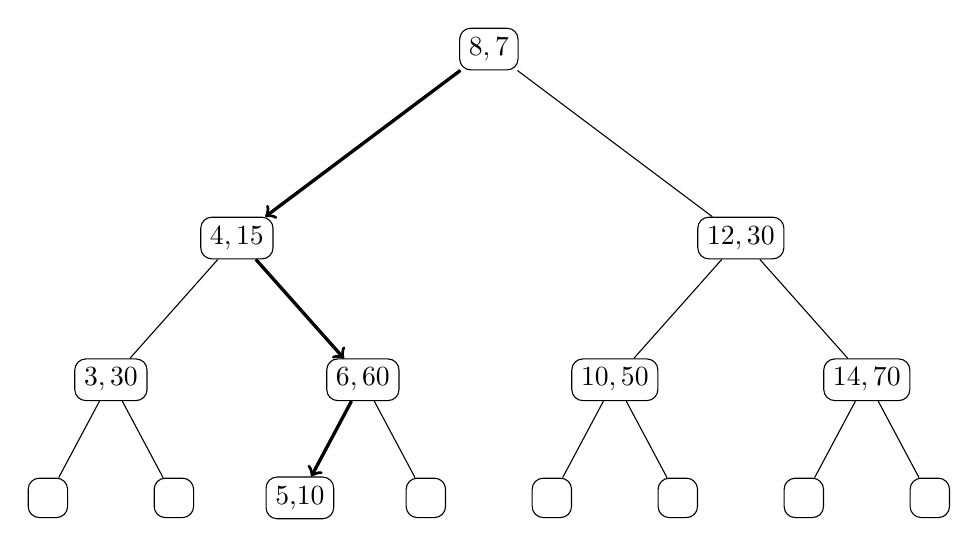
\begin{tikzpicture}[
minimum size=5mm,
level 1/.style={level distance=24mm,sibling distance=64mm},
level 2/.style={level distance=18mm,sibling distance=32mm},
level 3/.style={level distance=15mm,sibling distance=16mm},
every node/.style={draw,rounded corners}
]
\node (1){$8,7$}
child {
    node (2){$4,15$}
    child {
		node {$3,30$}
		child{node{}}
		child{node{}}
	}
    child {
		node (3){$6,60$}
		child{node(4){5,10}}
		child{node{}}
	}
}
child {
    node {$12,30$}
    child {
		node {$10,50$}
		child{node{}}
		child{node{}}
	}
    child {
		node {$14,70$}
		child{node{}}
		child{node{}}
	}
};

\draw[->,very thick] (1)--(2);
\draw[->,very thick] (2)--(3);
\draw[->,very thick] (3)--(4);
\end{tikzpicture}
\end{center}

The BST property holds, but the min-heap property is violated since $10<60$.

\begin{center}
\begin{tikzpicture}[
minimum size=5mm,
level 1/.style={level distance=24mm,sibling distance=64mm},
level 2/.style={level distance=18mm,sibling distance=32mm},
level 3/.style={level distance=15mm,sibling distance=16mm},
every node/.style={draw,rounded corners}
]
\node (1){$8,7$}
child {
    node (2){$4,15$}
    child {
		node {$3,30$}
	}
    child {
		node [fill=RED](3){$6,60$}
		child{node(4)[fill=RED]{5,10}}
		child [missing]
	}
}
child {
    node {$12,30$}
    child {
		node {$10,50$}
	}
    child {
		node {$14,70$}
	}
};

\end{tikzpicture}
\end{center}

\paragraph{Step 2: Rotation at $(6,60)$}

Strictly speaking rotation involves three nodes, so we imagine the right child of $(5,10)$ which is an empty 
node. We now perform a right rotation at $(6,60)$.

\usetikzlibrary{fit}

\begin{center}
\begin{tikzpicture}[minimum size=5mm, every node/.style={draw,rounded corners}]

\begin{scope}
\coordinate (a1) at (-1,1);
\coordinate (a2) at (0.2,0.1);
\node (b) at (1,-0.5) {$6,60$};
\node (c) at (-0.5,-2) {$5,10$};
\node (d) at (0.2,-3.2) {};
\node[
    draw,
    dotted,
    rounded corners,
    fit=(b)(c)(d),
    inner sep=8pt
] {};
\draw (a1)--(a2);
\draw (b)--(c);
\draw (c)--(d);
\end{scope}

\begin{scope}[xshift=8cm]
\coordinate (a1) at (-1,1);
\coordinate (a2) at (0.2,0.1);
\node (b) at (1,-0.5) {$5,10$};
\node (c) at (2.5,-2) {$6,60$};
\node (d) at (1.8,-3.2) {};
\draw (a1)--(a2);
\draw (b)--(c);
\draw (c)--(d);
\node[
    draw,
    dotted,
    rounded corners,
    fit=(b)(c)(d),
    inner sep=8pt
] {};

\end{scope}

\draw[->,thick] (3,-1.5)--(7,-1.5);


\end{tikzpicture}
\end{center}

The treap now becomes

\begin{center}
\begin{tikzpicture}[
level 1/.style={level distance=24mm,sibling distance=64mm},
level 2/.style={level distance=18mm,sibling distance=32mm},
level 3/.style={level distance=15mm,sibling distance=16mm},
every node/.style={draw,rounded corners}
]
\node {$8,7$}
child {
    node {$4,15$}
    child {node {$3,30$}}
    child {
        node {$5,10$}
        child[missing]
        child {node {$6,60$}}
    }
}
child {
    node {$12,30$}
    child {node {$10,50$}}
    child {node {$14,70$}}
};
\end{tikzpicture}
\end{center}



The heap property is still violated since $10 < 15$.

\begin{center}
\begin{tikzpicture}[
level 1/.style={level distance=24mm,sibling distance=64mm},
level 2/.style={level distance=18mm,sibling distance=32mm},
level 3/.style={level distance=15mm,sibling distance=16mm},
every node/.style={draw,rounded corners}
]
\node {$8,7$}
child {
    node [fill=RED]{$4,15$}
    child {node {$3,30$}}
    child {
        node [fill=RED]{$5,10$}
        child[missing]
        child {node {$6,60$}}
    }
}
child {
    node {$12,30$}
    child {node {$10,50$}}
    child {node {$14,70$}}
};
\end{tikzpicture}
\end{center}

\paragraph{Step 3: Rotation at $(4,15)$}

We imagine the left child of $(5,10)$ (which is an empty node) for the purposes of the rotation.

\begin{center}
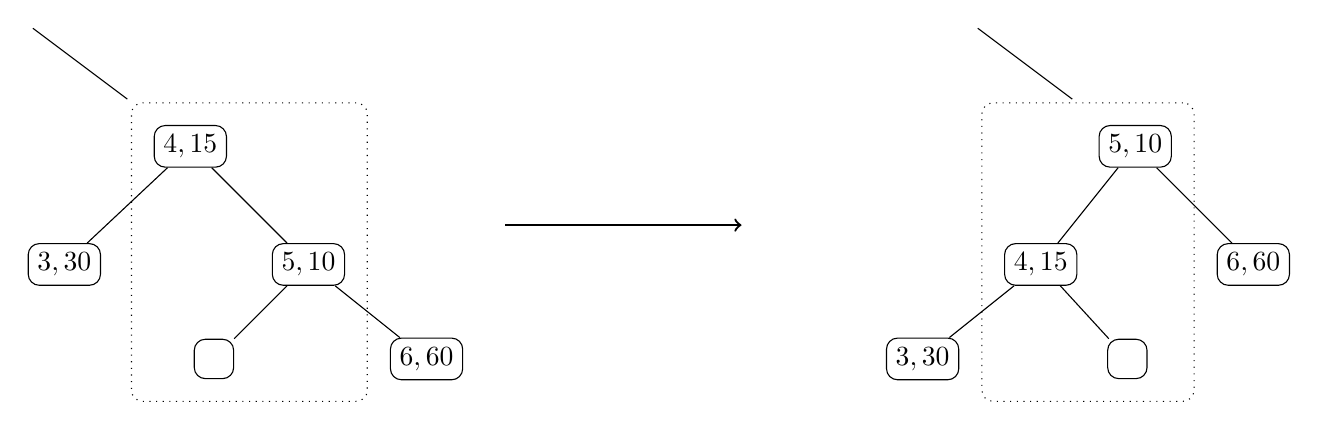
\begin{tikzpicture}[minimum size=5mm, every node/.style={draw,rounded corners}]

\begin{scope}
\coordinate (a1) at (-1,1);
\coordinate (a2) at (0.2,0.1);
\node (b) at (1,-0.5) {$4,15$};
\node (c) at (2.5,-2) {$5,10$};
\node (d) at (-0.6,-2) {$3,30$};
\node (e) at (4,-3.2) {$6,60$};
\node (f) at (1.3,-3.2) {};

\draw (a1)--(a2);
\draw (b)--(c);
\draw (b)--(d);
\draw (c)--(e);
\draw (c)--(f);

\node[
    draw,
    dotted,
    rounded corners,
    fit=(b)(c)(f),
    inner sep=8pt
] {};

\end{scope}

\begin{scope}[xshift=12cm]
\coordinate (a1) at (-1,1);
\coordinate (a2) at (0.2,0.1);

\node (b) at (1,-0.5) {$5,10$};
\node (c) at (-0.2,-2) {$4,15$};
\node (d) at (-1.7,-3.2) {$3,30$};
\node (e) at (2.5,-2) {$6,60$};
\node (f) at (0.9,-3.2) {};

\draw (a1)--(a2);
\draw (b)--(c);
\draw (c)--(d);
\draw (b)--(e);
\draw (c)--(f);
\node[
    draw,
    dotted,
    rounded corners,
    fit=(b)(c)(f),
    inner sep=8pt
] {};

\end{scope}

\draw[->,thick] (5,-1.5)--(8,-1.5);

\end{tikzpicture}
\end{center}


The heap property is now satisfied at every node:

\[
7 < 10,\qquad
10 < 15,\qquad
10 < 60,\qquad
30 < 50,\qquad
30 < 70.
\]

\begin{center}
\begin{tikzpicture}[
level 1/.style={level distance=24mm,sibling distance=64mm},
level 2/.style={level distance=18mm,sibling distance=32mm},
level 3/.style={level distance=15mm,sibling distance=16mm},
every node/.style={draw,rounded corners}
]
\node {$8,7$}
child {
    node {$5,10$}
    child {
        node {$4,15$}
        child {node {$3,30$}}
        child[missing]
    }
    child {
        node {$6,60$}
    }
}
child {
    node {$12,30$}
    child {node {$10,50$}}
    child {node {$14,70$}}
};
\end{tikzpicture}
\end{center}

The heap property is now satisfied at every node. Notice that it takes at most $\Theta(H)$ time to fix a 
violation since the violation always involves the inserted element and in each rotation its height 
increases by exactly one.

\subsubsection*{Search}
Searching in a treap is exactly the same as in a binary search tree -- at most $\Theta(H)$ time.

\subsubsection*{Deletion}
To delete an element, we must find it first. So we use the standard search to find it. Once it is found, 
we reverse the insert procedure by rotating \emph{down} until it becomes a leaf. Then we can safely 
delete it.

\section{Hash Tables}

The need arose for a data structure to store a set of elements with efficient search, 
insertion and deletion operations -- so we turn to hash tables!

\subsection{The Structure}

We begin with an empty array of size \(m\). Since this is a plain old normal 
array of size \(m\), we can access and modify 
any random element in constant time$\dots$

\begin{center}
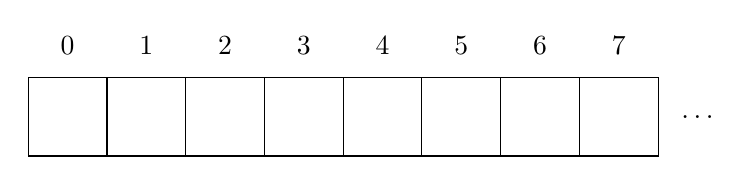
\begin{tikzpicture}
\foreach \i in {0,...,7}{
\draw (\i,0) rectangle (\i+1,1);
\node at (\i+0.5,1.4){\i};
}

\node at (8.5,0.5){$\dots$};
\end{tikzpicture}
\end{center}

\subsection{Insertion}
We add an element \(x\) by computing $i=\mathbf{H}(x)$. For example, 
suppose $\mathbf{H}(6)=3$. So we place \(6\) at index \(3\).


\begin{center}
\begin{minipage}{0.9\linewidth}
\begin{framed}
\begin{Verbatim}
Insert(x)
{
    i = H(x)
    traverse Linked_List[i]
    {
        if x present
            return
    }
    add x to end of Linked_List[i]
}
\end{Verbatim}
\vspace{-4mm}
\end{framed}
\end{minipage}
\end{center}

\paragraph{First insertion}

\begin{center}
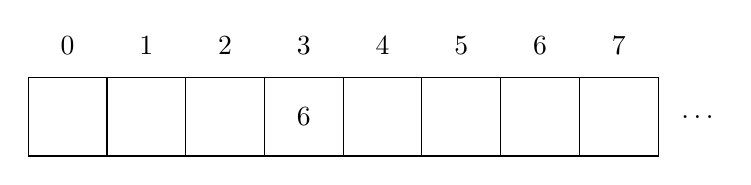
\begin{tikzpicture}
\foreach \i in {0,...,7}{
\draw (\i,0) rectangle (\i+1,1);
\node at (\i+0.5,1.4){\i};
}

\node at (8.5,0.5){$\dots$};

\node at (3.5,0.5){6};
\end{tikzpicture}
\end{center}

Similarly, we continue inserting elements in the same way as long as no two elements collide at the same index.

\paragraph{More insertions}

\begin{center}
\begin{tikzpicture}
\foreach \i in {0,...,7}{
\draw (\i,0) rectangle (\i+1,1);
\node at (\i+0.5,1.4){\i};
}

\node at (8.5,0.5){$\dots$};

\node at (1.5,0.5){4};
\node at (3.5,0.5){6};
\node at (5.5,0.5){11};
\node at (6.5,0.5){2};
\end{tikzpicture}
\end{center}

At this point, every index contains at most one element.

\paragraph{First \emph{collision}}

Now we attempt to insert \(7\). Suppose $\mathbf{H}(7)=3$.
We try to place \(7\) at index \(3\), but we find \(6\) already present.
So we extend that position into a linked list.

\begin{center}
\begin{tikzpicture}

% array
\foreach \i in {0,...,7}{
\draw (\i,0) rectangle (\i+1,1);
\node at (\i+0.5,1.4){\i};
}

\node at (8.5,0.5){$\dots$};

\node at (1.5,0.5){4};
\node at (3.5,0.5){6};
\node at (5.5,0.5){11};
\node at (6.5,0.5){2};

% arrow down
\draw[-{Latex}] (3.5,0) -- (3.5,-1);

% second element
\draw (3,-1) rectangle (4,-2);
\node at (3.5,-1.5){7};

\end{tikzpicture}
\end{center}

\paragraph{More collisions}

As more elements are inserted, collisions may occur at multiple indices, forming multiple linked lists.

\begin{center}
\begin{tikzpicture}

% array
\foreach \i in {0,...,7}{
\draw (\i,0) rectangle (\i+1,1);
\node at (\i+0.5,1.4){\i};
}

\node at (8.5,0.5){$\dots$};


\node at (1.5,0.5){4};
\node at (5.5,0.5){11};
\node at (6.5,0.5){2};

% chain at index 1
\node at (2.5,0.5){9};
\draw[-{Latex}] (1.5,0) -- (1.5,-1);
\draw (1,-1) rectangle (2,-2);
\node at (1.5,-1.5){14};
\draw[-{Latex}] (1.5,-2) -- (1.5,-3);
\draw (1,-3) rectangle (2,-4);
\node at (1.5,-3.5){21};

% chain at index 3 (our example)
\node at (3.5,0.5){6};
\draw[-{Latex}] (3.5,0) -- (3.5,-1);
\draw (3,-1) rectangle (4,-2);
\node at (3.5,-1.5){7};

\end{tikzpicture}
\end{center}

Thus, each index i stores a linked list of all elements 
inserted till now who hash to i. Let the total number of elements 
inserted be \(n\) and the number of indices be \(m\). Since on average 
each index has $\frac{n}{m}$ elements, the expected time of insertion 
is $\Theta(1+\frac{n}{m})$.

\subsection{Search}

\begin{center}
\begin{minipage}{0.9\linewidth}
\begin{framed}
\begin{Verbatim}
Search(x)
{
    i = H(x)
    traverse Linked_List[i]
    {
        if x found
            return true
    }
    return false
}
\end{Verbatim}
\vspace{-4mm}
\end{framed}
\end{minipage}
\end{center}

Since the expected number of elements per index is $\frac{n}{m}$, the 
expected time of search is $\Theta(\frac{n}{2m})$ since on average half the 
linked list is searched in a linear traversal.

\subsection{Deletion}
\begin{center}
\begin{minipage}{0.9\linewidth}
\begin{framed}
\begin{Verbatim}
Delete(x)
{
    i = H(x)
    traverse Linked_List[i]
    if x found
        remove x from Linked_List[i]
}
\end{Verbatim}
\vspace{-4mm}
\end{framed}
\end{minipage}
\end{center}

The expected time of deletion is $\Theta(\frac{n}{2m})$ since on 
average half the linked list is searched in a linear traversal.

Overall, the three operations are generally considered expected $\Theta(1)$ since we keep $n \le m$ and if 
$n$ exceeds $m$ we rehash with a larger $m$.

\section{Bloom Filters}

Suppose we wish to store a set of elements and support the operations 
\texttt{insert(x)} and \texttt{contains(x)}.
A straightforward solution is to store all inserted elements in an \texttt{unordered\_set}.
This gives expected $\Theta(1)$ insertion and lookup time, but requires memory proportional 
to the number of stored elements. When the number of elements becomes 
extremely large, memory itself may become the primary constraint. Bloom filters can achieve this tradeoff.

\subsection{The Structure}

Instead of storing the elements themselves, we store only a hash of the set. We begin with 
a bit array of size $m$ initialised to all zeros.

\begin{center}
\begin{tikzpicture}
\foreach \i in {0,...,7}{
\draw (\i,0) rectangle (\i+1,1);
\node at (\i+0.5,1.4){\i};
\node at (\i+0.5,0.5){0};
}

\node at (8.5,0.5){$\dots$};
\end{tikzpicture}
\end{center}

We then choose $k$ hash functions
\[
\left(H_1,H_2,\ldots,H_k\right)
\]
each mapping elements to the set of indices $\{0,1,\ldots,m-1\}$.

\subsection{Insertion}

To insert an element $x$, we compute
\[
\left(H_1(x),H_2(x),\ldots,H_k(x)\right)
\]

and set all corresponding bits to $1$. For example, if $k=3$ and the hash functions are $H_1(x)=3,\; H_2(x)=7,\; H_3(x)=10$
then we set positions $3,7,$ and $10$ of the bit array to $1$. If while inserting we see that a bit is already $1$, then we do nothing.\\


\noindent This operation is $\Theta(k)$ time.
\subsection{Search}

To determine whether an element $x$ is present, we again compute
\[
\left(H_1(x),H_2(x),\ldots,H_k(x)\right)
\]
and inspect the corresponding bits.
\begin{itemize}
\item If at least one of these bits is $0$, then $x$ was certainly never inserted.
\item If all of these bits are $1$, then we report that $x$ is present.
\end{itemize}
The second conclusion is of course subject to false positives! It is possible that the required bits 
were set earlier by completely different elements.\\


\noindent This operation is $\Theta(k)$ time.
\subsection{Utility of Bloom Filters}

The most important property of Bloom filters is that false negatives are impossible. If the filter 
reports that an element is absent, then that element was definitely never inserted. The only possible 
error is reporting that an element is present when it is actually absent.\\


Interestingly, Bloom filters (as the name suggests) are used as a filter. This means that incoming 
queries will go through the bloom filter -- if the element is absent, we can trust the result. Otherwise we can 
perform a more expensive lookup in the database. So it is useful to reduce the time taken to process a 
membership query.\\


\noindent It can be shown\footnote{See Problems!} that the error probability of a Bloom filter with 
optimal k is approximately $2^{-\frac{m\ln 2}{n}}$. For this to be small, we need $m$ to be large and $n$ to be small. But one might question, wasn't the 
whole point of the bloom filter to reduce the memory usage?\\

\noindent Let me clarify this with a practical example -- lets say we have a database of URLs. 
Each URL takes 100 bytes to store. Now let us say we have $10^9$ URLs -- and the deterministic \texttt{set} structure 
has a constant factor of about 10 per node in memory. So overall that would require $10^{12}$ bytes of memory which is about 1 TB.
In comparison, a Bloom filter of size $m=10\cdot n = 10^{10}$ bits would require only about 12.5 GB of memory.\\

\section{Cuckoo Hashing}
Recall that in ordinary hash tables, collisions are handled using linked lists. Cuckoo hashing takes a 
different approach. Instead of allowing multiple elements to occupy the same location, 
each element is given multiple possible locations and is stored in exactly one of
them.

\subsection{The Structure}

We maintain an array of size $m$ together with two hash functions $(H_1,H_2)$.

\begin{center}
\begin{tikzpicture}
\foreach \i in {0,...,7}{
\draw (\i,0) rectangle (\i+1,1);
\node at (\i+0.5,1.4){\i};
}

\node at (8.5,0.5){$\dots$};
\end{tikzpicture}
\end{center}

\subsection{Insertion}
Suppose we wish to insert an element $x$. Choose either of the hash functions $H_1$ or $H_2$ at random. 
Let this chosen hash be applied to $x$ to obtain an index $H(x)$. If the array is empty at that index, 
we are done. Otherwise, let the occupant be $y$. We evict\footnote{This behaviour resembles the cuckoo 
bird which lays its eggs in another bird's nest and kicks out the occupying eggs. Hence the name \dots} $y$ 
and place $x$ in its position. The displaced element $y$ must now be 
moved to its other possible location. If that position is occupied, 
another element is evicted, and the process continues.\\

\noindent We repeat this process until we either find an empty slot or find a 
cycle. 

\subsubsection*{Cycles and Rehashing}
In case we enter a cycle and insertion cannot be completed, choose new hash functions and 
rebuild the table from scratch. 

Note that overall, as long as we keep $n/m$ low, it can be shown that the expected time to 
insert an element is \(\Theta(1)\) average time similar to hash tables.
\subsection{Search}

To determine whether an element $x$ is present, we simply check the 
two possible locations $H_1(x)$ and  $H_2(x)$. If $x$ is found at either location, 
we report that it is present. Thus every lookup requires at most two array accesses, 
giving $\Theta(1)$ search time.

\clearpage
\section{Problems}

\begin{enumerate}
\item[\textbf{1}]
\begin{enumerate}[label=\textbf{(\alph*)}]
\item Prove that the expected search time in a skip list is \(\Theta(\log n)\). 
\textit{Hint: downward moves are bounded by height, which is expected \(\Theta(\log n\)).}

\item Deduce similarly that insertion takes expected \(\Theta(\log n)\) time.

\item Try inserting \(8\) into the following skip list using
 the procedure we described earlier:

\[
\begin{tikzpicture}[
x=1.8cm,
y=1.2cm,
>=Stealth,
every node/.style={font=\small}
]

\node[left] at (0,2) {Level 2:};
\node[left] at (0,1) {Level 1:};
\node[left] at (0,0) {Level 0:};

% Level 2
\node(a2) at (1,2) {1};
\node (e2) at (5,2) {9};

% Level 1
\node (a1) at (1,1) {1};
\node (c1) at (3,1) {5};
\node (e1) at (5,1) {9};

% Level 0
\node (a0) at (1,0) {1};
\node (b0) at (2,0) {3};
\node (c0) at (3,0) {5};
\node (d0) at (4,0) {7};
\node (e0) at (5,0) {9};

\draw[->] (a2) -- (e2);

\draw[->] (a1) -- (c1);
\draw[->] (c1) -- (e1);

\draw[->] (a0) -- (b0);
\draw[->] (b0) -- (c0);
\draw[->] (c0) -- (d0);
\draw[->] (d0) -- (e0);

\draw[->] (a2) -- (a1);
\draw[->] (a1) -- (a0);

\draw[->] (c1) -- (c0);

\draw[->] (e2) -- (e1);
\draw[->] (e1) -- (e0);

\end{tikzpicture}
\]

\item Can you think of a $\Theta(\log n)$ deletion strategy for skip lists?
\end{enumerate}

\item[\textbf{2}]
Consider n,m,k to be number of inserted elements, the size of bit array and the 
number of hash functions respectively in a Bloom filter. Assume the hash functions are independent.

\begin{enumerate}[label=\textbf{(\alph*)}]
\item Show that the probability of a particular bit in the array being set is $\left(1-\left(1-\frac{1}{m}\right)^{kn}\right)$ 
and thus the probability of a false positive is $\left(1-\left(1-\frac{1}{m}\right)^{kn}\right)^k$
\item Using suitable large m, n approximations, show that the optimal number of hash functions is $k=\frac{m}{n}\ln 2$
\item Put the above results together to show that the probability of a false positive is approximately $2^{-\frac{m\ln 2}{n}}$.
\end{enumerate}

\item[\textbf{3}]
Consider a Binary-Search Tree in which $n$ distinct elements are inserted in a random order. Without 
loss of generality, consider the elements to be $1,2,\ldots,n$. Let the random variable $H_i$ be the 
height when $i$ elements are inserted into the BST. Of course, $H_0=0$ and $H_1=1$.

\begin{enumerate}[label=\textbf{(\alph*)}]

\item Prove that $H_n \ge \log_2 (n+1)-1$
\item Use the definition of BST on the root to show that 

\[
(H_n | \; root=i) = 1+max(H_{i-1},H_{n-i})
\]

\item Use the substitution $Y_i = 2^{H_i}$ and take expectation both sides to show that 

\[
	\mathbb E[Y_n | \; root=i] = 2 \cdot \mathbb E[max(Y_{i-1},Y_{n-i})]
\]

\item Use the inequality $max(a,b) \le a+b$ and the law of total expectation to show that

\[
	\mathbb E[Y_n] \le \frac{4}{n} \cdot \sum_{i=1}^{n} \mathbb E[Y_{i-1}] 
\]


\item Substitute $S_n$ as the sum of $\mathbb E[Y_i]$ from $0$ to $n$ and show that 

\[
S_n \le S_{n-1} \left(1+\frac{4}{n}\right) 
\]

\item Use Telescoping Product and the value of $S_0 = \mathbb E[Y_0] = \mathbb E[2^{H_0}] = 1$ to show that 

\[
	S_n \le \binom{n}{4}
\]

\item Use the expectation form of Jensen's inequality and the result from \textbf{(f)} to show that 

\[
\mathbb E[H_n] \le \log_2 \left(\binom{n-1}{3}\right) 
\]

\item Use the result from \textbf{(a)} and \textbf{(g)} to show that 

\[
\mathbb E[H_n] = \Theta(\log n)
\]
\end{enumerate}
\end{enumerate}
